\documentclass[conference]{IEEEtran}
\IEEEoverridecommandlockouts
% The preceding line is only needed to identify funding in the first footnote. If that is unneeded, please comment it out.
\usepackage[dvipsnames]{xcolor}
\usepackage{cite}
\usepackage[most]{tcolorbox}
\usepackage{amsmath,amssymb,amsfonts,amsthm}
\usepackage{algorithmic}
\usepackage{graphicx}
\usepackage{subcaption}
\usepackage{textcomp}
\usepackage{mathtools}
\usepackage[shortlabels]{enumitem}
\usepackage{xspace}
\usepackage{listings}
\usepackage{fontenc}


%% PL packages
\usepackage{stmaryrd} 
\usepackage{proof}
\usepackage{mathpartir}
\usepackage{color}
\usepackage{xstring}

\def\BibTeX{{\rm B\kern-.05em{\sc i\kern-.025em b}\kern-.08em
    T\kern-.1667em\lower.7ex\hbox{E}\kern-.125emX}}
\definecolor{darkblue}{rgb}{0,0,0.5}
\definecolor{darkgreen}{rgb}{0,0.3,0}
\definecolor{darkpink}{rgb}{0.4,0,0.3}
\definecolor{graygreen}{rgb}{0.3,0.5,0.3}
\definecolor{grayblue}{rgb}{0.2,0.2,0.6}
\definecolor{grayred}{rgb}{0.5,0.2,0.2}

\lstset{
  backgroundcolor=\color{white},     % choose the background color; you must add \usepackage{color} or \usepackage{xcolor}; should come as last argument
  % identifierstyle=\color{red},
  basicstyle=\footnotesize\ttfamily\upshape,      % the size of the fonts that are used for the code
  breakatwhitespace=false,              % sets if automatic breaks should only happen at whitespace
  breaklines=false,                     % sets automatic line breaking
  captionpos=b,                         % sets the caption-position to bottom
  abovecaptionskip=-3 mm,
  commentstyle=\itshape\color{graygreen}, % comment style
  % escapeinside={(:}{:)},             % if you want to add LaTeX within your code
  escapechar={!},
  % extendedchars=true,              % lets you use non-ASCII characters; for 8-bits encodings only, does not work with UTF-8
  % firstnumber=1000,                % start line enumeration with line 1000
  % frame=tb,                        % adds a frame around the code
  % keepspaces=true,                 % keeps spaces in text, useful for keeping indentation of code (possibly needs columns=flexible)
  keywordstyle=\color{blue},     % keyword style
  language=Haskell,                  % the language of the code
  morekeywords={ forMseq_, generate, forAllM, fork, forever }
  %morekeywords={ Set, Tree, Leaf, Node, Applicative, fmap, liftA2, bimap, foldMap
  %             , traverse, mappend, pure, Foldable, Traversable, zero, one
  %             , Semiring, Semigroup, NonEmpty, sconcat, TSet,
  %             , SimplicialSet, TSimplicialSet, Graph, TGraph, LGraph
  %             , Map, IsString, fromString },
  deletekeywords={instance, data, where, class, filter, type, insert, delete, union, map},      % if you want to delete keywords from the given language
  emph={data, class, instance, where, type},
  emphstyle=\color{darkpink},
  numbers=none,                      % where to put the line-numbers; possible values are (none, left, right)
  % numbersep=5pt,                   % how far the line-numbers are from the code
  % numberstyle=\tiny\color{mygray}, % the style that is used for the line-numbers
  % rulecolor=\color{black},         % if not set, the frame-color may be changed on line-breaks within not-black text (e.g. comments (green here))
  % showspaces=false,                % show spaces everywhere adding particular underscores; it overrides 'showstringspaces'
  % showstringspaces=false,          % underline spaces within strings only
  % showtabs=false,                  % show tabs within strings adding particular underscores
  % stepnumber=2,                    % the step between two line-numbers. If it's 1, each line will be numbered
  stringstyle=\color{grayred},     % string literal style
  % tabsize=2,                       % sets default tabsize to 2 spaces
  % title=\lstname                   % show the filename of files included with \lstinputlisting; also try caption instead of title
  xleftmargin=10pt,
  aboveskip=8pt,
  belowskip=4pt
}

\begin{document}

\usetikzlibrary{matrix, arrows.meta, calc, positioning}
\tikzset{myarrow/.style={-Latex, rounded corners},}

\definecolor{vert}{RGB}{0,181,0}
\definecolor{oran}{RGB}{223,74,0}
\definecolor{viol}{RGB}{134,0,175}
\definecolor{roug}{RGB}{215,15,0}
\definecolor{bb}{RGB}{0,0,0}
\definecolor{gg}{RGB}{220,220,220}

\newtcolorbox[auto counter]{bbox}[2][]{%
    colback=white,
    colframe=bb,
    boxrule=1pt,
    %colbacktitle=white!90!roug,
    colbacktitle=white!40!gg,
    coltitle=black,
    fonttitle=\footnotesize\bfseries, 
    fontupper=\footnotesize,
    fontlower=\footnotesize,
    enhanced,
    sharp corners,
    attach boxed title to top left={yshift=-2mm, xshift=0.5cm},%
    #1,% For possible options
}
\title{SAUCy: Super Awesome Universal ComposabilitY }

\newcommand{\mc}[1]{\ensuremath{\mathcal{#1}}}
\newcommand{\msf}[1]{\ensuremath{{\mathsf {#1}}}}
\newcommand{\mathc}[1]{\ensuremath{\mathcal{#1}}}
\newcommand{\tsc}[1]{\textsc{#1}}
\newcommand{\f}[1]{\ensuremath{\mathcal{#1}}\xspace}
\newcommand{\F}{\f{F}}
\newcommand{\PI}{\ensuremath{\pi}\xspace}
\newcommand{\RHO}{\ensuremath{\rho}\xspace}
\newcommand{\achan}{\ensuremath{\F_{\msf{achan}}^{p_r,p_s}}}
%\newcommand{\C}{\mathcal{C}}
\newcommand{\con}[1]{\msf{Contract_{#1}}}
%\newcommand{\Fsync}[2]{\ensuremath{\F_{\msf{sync},#1,#2}}}
\newcommand{\Fsync}[2]{\ensuremath{\F_{\msf{BD-SEC}}(#1,#2)}}
\newcommand{\Fchan}[2]{\ensuremath{\F_{\msf{chan}}(#1,#2)}}
\newcommand{\Fbdsec}{\ensuremath{\F_{\msf{BD-SEC}}^{\delta,\ell}}}
\newcommand{\Fbc}{\ensuremath{\F_{\msf{broadcast}}}}
\newcommand{\Fsfe}{\ensuremath{\F_{\msf{SFE}}}}
\newcommand{\Fstate}{\ensuremath{\F_{\msf{state}}}}
\newcommand{\Fclock}{\ensuremath{\F_{\msf{clock}}}}
\newcommand{\Frbc}{\ensuremath{\F_{\msf{rbc}}}}
\newcommand{\Fpay}{\ensuremath{\F_{\msf{pay}}}}
\newcommand{\Fcom}{\ensuremath{\F_{\msf{com}}}\xspace}
\newcommand{\Fauth}{\ensuremath{\F_{\msf{auth}}}\xspace}
\newcommand{\Fflip}{\ensuremath{\F_{\msf{coinflip}}}\xspace}
\newcommand{\Fro}{\ensuremath{\F_{\msf{RO}}}\xspace}
\newcommand{\Fsmc}{\ensuremath{\F_{\msf{SMC}}}\xspace}
\newcommand{\Fropp}{\ensuremath{\F_{\msf{P2P\hyp RO}}}\xspace}
\newcommand{\Gledger}{\ensuremath{\f{G}_{\msf{ledger}}}}
\newcommand{\Wsync}{\ensuremath{\mathcal{W}_{\msf{sync}}}}
\newcommand{\Wasync}{\ensuremath{\mathcal{W}_{\msf{async}}}}
\newcommand{\Ssyncbracha}{\ensuremath{\mathc{S}_{\msf{sbracha}}}}
\newcommand{\Fbracha}{\ensuremath{\mathcal{F}_{\msf{bracha}}}}
\newcommand{\Schedule}{\tsc{Schedule}}
\newcommand{\Delay}{\tsc{Delay}}
\newcommand{\Advance}{\tsc{Advance}}
\newcommand{\Exec}{\tsc{Exec}}
%\newcommand{\Adversary}{\ensuremath{\mathcal{A}}\xspace}
\newcommand{\A}{\ensuremath{\mathcal{A}}\xspace}
\newcommand{\DummyAdv}{\ensuremath{\mathcal{A}_\mathcal{D}}\xspace}
\newcommand{\DA}{\ensuremath{\A_\mathcal{D}}\xspace}
\newcommand{\Sim}{\ensuremath{\mathcal{S}}\xspace}
\newcommand{\SIM}[1]{\ensuremath{\mathcal{S}_{#1}}\xspace}
\newcommand{\simcom}{\SIM{\msf{com}}}
\newcommand{\cf}{\ensuremath{\mathcal{C}}\xspace}
\newcommand{\ID}[1]{\ensuremath{\mathcal{I}(#1)}\xspace}
%\newcommand{\Sim}[1][]{\ifthenelse{\equal{#1}{}}{\ensuremath{\Simulator}}{\ensuremath{\Simulator_{#1}}}}
\newcommand{\DS}{\SIM{D}\xspace}
%\newcommand{\Environment}{\ensuremath{\mathcal{Z}}\xspace}
\newcommand{\Z}{\ensuremath{\mathcal{Z}}\xspace}
\newcommand{\Partyi}{\ensuremath{P_i}}
\newcommand{\Partyj}{\ensuremath{P_j}}
\newcommand{\partywrapper}{multiplexer\xspace}
\newcommand{\pw}{\PI}
\newcommand{\fwrapper}{\todo{fwrappername}\xspace}

\newcommand{\dealer}{\ensuremath{\mathcal{D}}}
\newcommand{\globalf}[1]{\ensuremath{{\overline{\mathcal{#1}}}}}
\newcommand{\todo}[1]{\textcolor{Red}{todo: #1}}
\newcommand{\edict}{\{\}}
\newcommand{\lar}{\leftarrow}
\newcommand{\rar}{\rightarrow}
\newcommand{\Init}{{\bf \color{NavyBlue} Init}~}
\newcommand{\OnInput}{{\bf \textcolor{Black} On input}~}
\newcommand{\Allinputs}{{\bf \color{Cerulean} All other input~}}
\newcommand{\OnAdvInput}{{\bf \color{BrickRed} On input}~}
\newcommand{\heading}[1]{\textbf{#1}}
\newcommand{\Type}{\ensuremath{\yo{type}}}
\newcommand{\Stype}{\ensuremath{\yo{stype}}}
\newcommand{\bangf}{\ensuremath{!\F}}
\newcommand{\execuc}{\ensuremath{\msf{execUC}}}
\newcommand{\iexecuc}{\inline{execUC}}
\newcommand{\UC}[4]{\ensuremath{\execuc #1  #2  #3  #4}}
\newcommand{\idealP}{\ensuremath{\mathbbm{1}_d}\xspace}
%\newcommand{\prot}[1][]{\ifthenelse{\equal{\ensuremath{#1}}{}}{\ensuremath{\Pi}}{\ensuremath{\Pi_{X #1}}}}
\newcommand{\prot}[1]{\ensuremath{\pi_{\msf{#1}}}}
\newcommand{\lla}{\leftarrow}
\newcommand{\lvd}{\vdash}
\newcommand{\tb}[1]{\text{\color{royalblue}{#1}}}
\newcommand{\tgr}[1]{\text{\color{forestgreen}{#1}}}
\newcommand{\tm}[1]{\text{\color{magenta}{#1}}}
\newcommand{\tg}[1]{\text{\color{gray}{#1}}}
\newcommand{\tp}[1]{\text{\color{purp}{#1}}}
\newcommand{\nparam}[1]{\tp{#1}}
\newcommand{\tr}[1]{\text{\color{Red}{#1}}}
\newcommand{\yo}[1]{\text{\color{YellowOrange}{#1}}}
\newcommand{\inline}[1]{\lstinline[basicstyle=\footnotesize\BeraMonottFamily, mathescape]!#1!}
\newcommand{\nrecv}{\tb{recv}}
\newcommand{\nsend}{\tb{send}}
\newcommand{\nget}{\tb{get}}
\newcommand{\npay}{\tb{pay}}
\newcommand{\nsimget}{\tm{simget}}
\newcommand{\nsimpay}{\tm{simpay}}
\newcommand{\ncase}{\tm{case}}
\newcommand{\nproc}{\tb{proc}}
\newcommand{\nwithdraw}{\tm{withdrawTokens}}
\newcommand{\nif}{\yo{if}}
\newcommand{\nthen}{\yo{then}}
\newcommand{\nend}{\yo{end}}
\newcommand{\nwhile}{\yo{while}}


%\newcommand{\pluseq}{\mathrel{+}=}
%\newcommand{\minuseq}{\mathrel{-}=}
\newcommand{\Assert}{{\bf \color{BrickRed} Assert }}
\newcommand{\Require}{{\bf \color{BrickRed} Require }}

%\theoremstyle{acmdefinition}
%\newtheorem{definition}{Definition}[section]
\newtheorem{ddef}{Definition}
%\newtheorem{theorem}{Theorem}
\newtheorem{claim}{Claim}
%\newtheorem{lemma}{Lemma}

%\newlist{renumerate}{enumerate}{1}
%\setlist[renumerate]{before=\setlength{\baselineskip}{20pt}, itemsep=-2ex, topsep=-2ex}
%\newenvironment{renumerate}{\begin{enumerate}[before=\setlength{\baselineskip}{20pt},itemsep=-2ex,topsep=0pt]}{\end{enumerate}}
\newenvironment{renumerate}{\begin{enumerate}[nosep]}{\end{enumerate}}
%\newenvironment{ritemize}{\begin{itemize}[before=\setlength{\baselineskip}{20pt},itemsep=-2ex,topsep=0pt]}{\end{itemize}}
\newenvironment{ritemize}{\begin{itemize}[nosep] \renewcommand\labelitemi{--}}{\end{itemize}}

\newenvironment{mylst}{\begin{lstlisting}[basicstyle=\small\BeraMonottFamily, frame=single, mathescape]}{\end{lstlisting}}

\makeatletter
\newcommand{\inmsg}[1]{%
(#1\checknextarg}
\newcommand{\checknextarg}{\@ifnextchar\bgroup{\gobblenextarg}{)~}}
\newcommand{\gobblenextarg}[1]{, #1\@ifnextchar\bgroup{\gobblenextarg}{)~}}
\makeatother


\newcommand{\transfermsg}{\inmsg{transfer}{to}{val}{data}{from}}
\newcommand{\createmsg}{\inmsg{contract \ create}{addr}{val}{data}{private}{from}}
\newcommand{\reject}{\textbf{reject}~}
\newcommand{\ignore}{\textbf{ignore}~}
%\newcommand{\For}{\textbf{For}~}
\newcommand{\Env}{\ensuremath{\mathcal{Z}}}
%\newcommand{\While}{\textbf{While}~}
\newcommand{\Buffer}{\textbf{Buffer}~}
\newcommand{\Send}{\textbf{Send}~}
\newcommand{\Output}{\emph{Output}~}
\newcommand{\Leak}{\textbf{Leak}}
\newcommand{\Eventually}{\textbf{Eventually}~}
\newcommand{\In}{\textbf{in}~}
\newcommand{\If}{\textbf{If}~}
\newcommand{\Else}{\textbf{Else}~}
%\newcommand{\Return}{\textbf{Return}~}

\newcommand{\pluseq}{\ensuremath{\mathrel{+}=}}
\newcommand{\minuseq}{\ensuremath{\mathrel{-}=}}
\newcommand{\Adv}{\ensuremath{\mathcal{A}}}
%\newcommand{\Partyi}{\ensuremath{\mathbf{P_i=(sid,pid)}}}
\newcommand{\sid}{\ensuremath{\msf{sid}}\xspace}
\newcommand{\pid}{\ensuremath{\msf{pid}}\xspace}
\newcommand{\dquad}{\quad \quad}
\newcommand{\qqquad}{\qquad \quad}
\newcommand{\qqqquad}{\qqquad \quad}
\newcommand{\qqqqquad}{\qqqquad \quad}

\newcommand*\circled[1]{\tikz[baseline=(char.base)]{
            \node[shape=circle,draw,inner sep=1pt] (char) {#1};}}

\newcommand*\token{~\circled{t}}

\DeclarePairedDelimiter{\ceil}{\lceil}{\rceil}


\newcommand{\spheading}[1]{ %
	\rotatebox{60}{\parbox{2.5cm}{\raggedright #1}}}


\author{\IEEEauthorblockN{Anon}
\IEEEauthorblockA{\textit{Nowhere}}
}

\maketitle

\begin{abstract}
% UC standard for cryptography and used in defining distributed systems as well, especially in the current era of asynchronous blockchain protocols
% UC is esoteric, hard to understand, and not useful to programmers despite its appeal to modularity
% even proofs/code in literature is implemented in a non-UC way so security proofs become kind of useless
% existing tooling makes proving easier but tranfers the problem to working with bespoke languages, foralisms, etc.

The UC framework is a well-known proving framework for cryptographic protocols, and more recently distributed protocols, in the academic community.
Decentralized protocols, namely blockchain protocols, rely on layers of distributed asynchronous protocols with different fault models and guarantees, and, despite UC's success the framework rarely makes its way outisde of academic circles in such settings.
This results from its highly technical nature which makes it difficult to understand by those not already familiar, and its predominant use for cryptographic protocols which require much greater care in implementation that the framework isn't, yet, equipped to handle~\footnote{As opposed to distributed protocols, implementations of a cryptographic primitives requires careful consideration of memory access patterns, side channel leaks, computer architecture, etc.} compared to the needs to asynchronous distributed protocols that assume cryptographic primitives. 

Programming languages and tooling exists for UC to aid in autmating proving, but do little to make UC more accessible in practice. Instead, they add additional layers of complexity by requiring learning new languages and formalisms.
We content that UC can be useful as a software development framework, and that is modularity and composability guarantees can benefit the development of distributed asynchronous protocols.
The framework's security definition, as a relation to an idealized program, allows for simpler expression of properties useful in distributed settings, like adverasrial influence and fairness, espcially where financial incentives are involved. 

\todo{roadblocks to UC, the UC real-ideal relation, we can use that to detect many classes of common bugs, better modelling for async in order to help reason about liveness, but negative result here}

The UC framework is the gold standard for proving the security of cryptographic and distributed protocols, however its highly technical nature makes it difficult to understand and use for those not already well-versed.
This renders on-paper proofs and costructions hard to verify or understand, and it results in implementations of such protocols departing from the UC computation model alltogether rendering security prooff obsolete.
Existing programming language tools for UC attempt to make proving and writing definitions easier through a type systems and applying formal verification, but do little to make UC more accessible by introducing bespoke programming languages and formalisms.

We contend that UC has a place as software develpoment framework, and not only a theoretical proving framework.
Specifically, its modularity and compositional security guarantees suggest it aligns well with fundamental software development principles, and it's ideal functionality model succintly captures intended properties, adversarial capabilities, and stands are a more specfic and useful analog of a software module.
\todo{we want to show that UC is amenable to software engineering and challenge conventional wisdom and say that this avenue requires greater work/effort/investiation/research where the payoff could be great!}

We validate this claim by proposing a simpler, more programmining-friendly, abstraction to network modelling in UC and through case studies to understand how well UC works with existing software practicies.
Specifically we use fuzz testing as our experimental apparatus, and apply it to implementations of real byzantine agreement protocols ranging from simple to complex. 
We demonstrate the usefulness of the ideal functionality definitions as a high-level property-based models, UC's adversarial modelling of scheduling and leaks for testing protocol paths, and the advantage of its modular approach on minimizing state space for fuzzers. 

\todo{how to throw in that along the way we arrive at a few insights into what it means to write code or on-paper definitions in the UC-style and how it manifests itelf (like multi-threaded computation model vs ITM model)}
\end{abstract}

\begin{IEEEkeywords}
component, formatting, style, styling, insert
\end{IEEEkeywords}

\section{Introduction}
% RESEARCH QUESTIONS:
%     (RQ1). Is UC suitable and practical as a development framework rather than only a theoretical framework?
%             (i). Can existing UC models/techniques be improved for an engineering purpose?
%             (ii). What are the advantages of using UC for development?
%     (RQ2). Is UC as a development framework compatible with existing informal analysis techniques?
%             (i).  Fuzz testing is widely used, is a successful analysis tool, and is itself an engineering undertaking. Can we successful apply fuzzing to UC?
%             (ii).  Does the ideal functionality model and out realization of import aid in analyzng liveness in distributed protocols?

Universal composability is the leadeding framework for defining the security of message-passing cryptographic protocols between mutually distrustful parties.
Though largely used for cryptography, it has seem a reemergence in asynchronous distributed systems literature, especially due to the rise of decentralized protocols where applications are a composition of many interacting layers of other asynchronous distributed systems with different fault models and properties.
This highly compositional nature, combined with a new setting where financial incentives make properties like fairness, output distribution, and adversarial influence more relevant, have led to increasing interest in UC for distributed protocols.
At its core the framework's appeal is that it allows protocols to be designed in isolation and rely on idealized versions of other subprotocols and assumptions that behave like trusted third parties--called \emph{ideal functionalities}. 
It security definition allows proving of protocols, also in isolation, while ensuring that the proof holds when ideal functionalities are replaced with real protocols and the protocol is composed with arbitrarhy other protocols. 
Far from only a theoretical framework, this form of design and security definition lends itself well to the this setting.
%The UC composition operator and security definition allows replacing ideal functionalities with protocols that realize them (in isolation) to realize a larger protocol. 

The real-ideal paradigm plays a big role in the success and usefulness of the framework, because it allows defining the properties and security of a protocol through a single relation of indistinguishability with a protocol.
Comparing to an idealized program allows for expressing arbitrarily complicated and intertwined properties that can be cumbersome and error-prone with property-based definitions, i.e. a laundry list of assertions that must hold. 
In the earliest formulation of the framework, a simple two party computation (2PC) is described where the properties of secrecy and correctness are closely related, especialy in the byzantine setting when attempting to quantify how adversaries choose inputs, their influence on outputs, output fairness, and adversarial knowledge.
Expressing and analyzing these properties is crucial to meaningfully realize UC security, especially in the aforementioned world of decentralized protocols.
We proposet the following concrete research questions:
\begin{enumerate}[label=RQ\arabic*.]
\item Is the real-ideal paradigm useful even in identifying implementation-level bugs, and performing test cases analysis for protcol security?
\item Can UC implementation express and analyze protocols that express such properties and whether they hold in isolation and across layered and parallel composition?
\end{enumerate}
The real-ideal relationship is about testing generation against all environemnts, therefore, we select fuzz testing as our method for examing these two research questions. 
Not only is fuzzing a natural choice for testing the real-ideal relationship, but showing that we can meaningfully use such an important widespread tool in UC lends credence to our claim of UC as a candidate as a development framework. 
We use this tool to analyze a range of asynchronous protocols and idenfity implementation-level bugs that manifest themselves as distinguishing environments.

\todo{also do coin flipping under composition}

\todo{state why we need to do this for async because existing practices seem to fall short of doing this kind of analysis for them}


We believe that these advantages and features of UC mdoelling are specifically advantageous for asynchronous distributed protocol, and, in this work, we explore whether they can be realized as a software development framework using informal analysis techniques.


%\item Is UC suitable and practical as a development framework rather than only a theoretical one?
%    \begin{itemize}
%        \item [(i)] Can existing UC models/techniques be improved for easy of development?
%        \item [(ii)] What are the advantages of using UC for development?
%    \end{itemize}
%\item Is UC compatible with existing software analysis techniques?
%    \begin{itemize}
%        \item [(i)] Does the ideal functionality model and UC's polynomial time notion aid in reasoning about liveness in implementations?
%    \end{itemize}
%\todo{Hypotheses: why UC for async protocols and distributed systems are where this matters the most}
%
%\todo{maybe something along these lines: good as a dev framework for analyzing security and better researcher tooling for analyzing definitions without cumbersome extra work}.

There is a large amount of exsisting literature proposing programming language (PL) and formal verification tools for expressing UC security in limited, but useful ways~\cite{.}.
Contrary to our goal, working with new process calculi, a new domain-specific language, or a proving framework do little to make UC more accessible to non-cryptography researchers because 
\begin{enumerate}
\item Niche programming languages aren't well-suited to production environments and add to the already high learning curve.
\item The added obligations of using PL machinery for mechanizing proofs can add significant work for researchers as well~\cite{ironfleet,easycryptuc} \plan{easycrypt requires a whole new method of communication that makes translating definitions annoying} \todo{saying ``can add burden'' is an unproven claim but maybe still okay?}
\end{enumerate}

For researchers, software artefacts are a crucial for establishing more precise definitions that a broader audience can interact with, resuse, and rigorously test. 
Engineering aside, opening research up to broader falsiability of definitions/proofs is important.
For software engineers, there is a clear advanage to implementing code that matches academic definitions, the ideal functionality models provides a clear interface (specification, adversarial capabilities, and security guarantees) for software modules, and a UC environment facilitates more sophisticated protocol analysis because of its exposure to both honest party input/output and adversarial action.\todo{the point is along the lines mentioned that both scheduling and inputs/outputs allow more intelligent choice of actions for testing more interesting conditions...}
Simply put, UC is an efficient \todo{efficient?} harness for developing and testing protocos under byzantine conditions.
Furthremore, maintaining a symmetry between paper definitions and the resulting implementation solidifies the validity of existing security proofs.

\todo{maybe mention mainstream language earlier}
In order to address our research questions, and intuition, about UC, we implement it in a mainstream language, Haskell, and apply fuzz testing as our candidate analysis technique to explore UC's suitability as a development framework for distributed protocols.
Fuzz testing is a method of property-based testing that involves generating random inputs and checking output against a spec, and prior work shows that it can be as successful, if not better, than formal approaches like symbolic execution. 
It is widely used in practice and considered to be a vital tool in software testing.
Furthermore, implementing fuzzing is itself an engineering excercise that tests the framework's flexibility. 
Additionally, we propose a new mechanism for capturing an asynchronous network that extends asynchronous message deliver to asynchronous code execution. 
Our mechanism, an asynchronous wrapper, allows ITMs to schedule code blocks whose execution is controlled by the adversary and uses the new import mechanism for polynomial time to achieve eventual delivery~\footnote{The import mechanism was devised to overcome problems with previous versions of polytime like the ``length-of-input'' notion, and, as far as we know, we are the first to use it in this way}.
Moving away from traditional definitions that only work with messages, \emph{eventually} executing code blocks massively simplifies UC definitions and is an abstraction familiar to software engineers in other programming languages.
\plan{In fact, we posit that there is significant room for innovation on similar conventional UC-isms.}



We validate this vision for UC by implementing it in a mainsteam language and studying its compatibility with existing development practices. 
\todo{sopped edit here, te rest is not edited:} This implementation realizes the ITM computation model, and provides type checking of channel interfaces between module though we envision more descriptive type systems can be applied to this task.
We push modular and programming-inspired UC designs further by providing a new abstraction for realizing asynchronous, and other arbitrary, networks that both greatly simplifies paper-and-pencil definitions/proofs and an \emph{asynchronous code} abstraction familiar to programmers.
Finally, we employ fuzz testing, a critically important and highly successful testing strategy in modern software engineering, to our own implementations of canonical and modern byzantine agreement protocols and showcase
\begin{itemize}
\item the UC framework especially lends itself to fuzz testing by reducing complex distributed systems to a set of simple protocol and adversarial interfaces that greatly reduce the input space to be searched
\item the real/ideal paradigm already provides a built-in specification, the ideal functionality, of the inteded protocol to test protocols properties against
\item our novel design of asynchronous computing/networking \todo{something something}
\end{itemize}

Rough notes for the paragrapph. 
We implement bracha, ben-or, aba and inject faults into them. show how simple fuzzers that don't target specific vulnerabilities can find bugs that violate agreement/safety/etf
the better approach might be to idenftify only the set of bugs that would induce failures in safety and then say that those can be identified
but what about simpler bugs? that would require more meaningful testing but not what UC is good fr
existing fuzz testing is already good for bugs in single compiled progra like a single protocol running in isolation, so we don't think of finding those
but finding those of a distributed nature


Rather than bridge the gap between cryptography reserachers and protocol implementers, these approaches aid validation but accept and embrace the complexity of the framework.
Ultimately, the advantages of the proving framework, and the paper proofs that rely on it, are lost because of code that completely departs from them. 




%  Universal Composability (UC)~\cite{canettiUC} is the leading framework for defining security properties of cryptographic protocols.
%  It is considered the strongest definitional model since it guarantees the security properties hold even when the protocol is arbitrarily composed with
%  multiple concurrently-executing sessions of other protocol.
%  UC has gained popularity for analyzing cryptographic protocols due to its \emph{ideal world/real world} simulation mechanism.
%  In contrast to game-based cryptography where security properties are defined via attack games,
%  UC defines the \emph{ideal functionality}, a trusted third party that serves as the \emph{protocol specification}.
%  A core feature of the frameowk is its modularity where complex protocols are defined in terms of simple, ideal functionality building blocks that are secure by definition. 
%  A major drawback of UC is that security proofs can be quite complicated and difficult to analyze. 
%  Many related works \cite{ilc, easyuc, ipdl, etc} attempt to formalize UC security through a new programming language or defining UC security in an existing formal verification lanuage, and,  
%  although useful, such tools frequently never make their way to software engineering practice because
%  1. niche programming languages aren't suited to large scale development and can be difficult to use, and 2. the added proof obligations on the programmer can be extensive~\cite{ironfleet}.
%  Utimately, UC-secure prtocols end up being implemented in software frameworks that do not replicate UC, and, therefore, my invalidate on-paper proofs without further security proofs of the code.
%  
%  We address this gap in UC-driven software develoment by exploring how inforal security analysis of UC definitons, in our implementation of UC, can identify, and aid in eliminating, security vulnerabilities.
%  A key controbution of our software development framework for UC is proposing a noval new abstraction for capturing network assumptions. Our abstraction makes use of the novel import mechanism 
%  for polynomial time and fits nicely as a software abstraction. Our implementation and network model are, to the best of our knowledge, the first concretiziations of the import mechanism in this way.
%  Prior attempts at modelling asynchrnous networks, for example, focus primarily on adversarial delay of messages between parites. Such notions can require
%  protocols to encode signficant model-specific behavior which clutters functionalitiy (and protocol) definitions, places unecessary restrictions on protocol design, and is counter-productive for modular and reusable code. 
%  Out abstraction, on the other hand, acts are a wrapper around ITMs and offers a notion of \emph{asynchronous computation} in a way that is UC-compatible and firs well within a software framework. 
%  Not only is it natural for software development, but it also reduces functionality and protocol code to be almost model-agnostic. 
%  We use our network model of computation to focus solely on modeling and analzing distributed protocols in this work.
%  UC is most notably a framework for cryptographic protocols, however, in recent years the emergence of decentralized systems has renewed focus on modelling the security of asynchronous byzantine networks in UC~\cite{many,cit,ations}. 
%  Decentralized, namely blockchain, systems are highly modular with many protocols sharing state in unexpected ways and relying on numerous shared distrbuted sub protocols.
%  Naturally, compositional security in UC is ideal for capturing such protocols. 
%  
%  We opt for fuzz testing, by generating environments, as our analysis tool for three important reasons. First, numerous prior work has demonstrated the success of fuzz testing at identifyin software bugs. 
%  Some work suggests fuzzing is comparable in success to even formal approach such as symbolic execution. 
%  Second, the UC framework lends itself to compact definitions that compose through ideal functionalities making the input space for protocol parties and adversaries much smaller. 
%  Combined with our simple network model, UC modularity makes it easier for generated environmenst to explore more of the state space for a particular protocol or simulator proof. \todo{is this setting us up with an obligation to prove this statement with some coverage testing?}
%  Third, the real/ideal paradigm, and the ideal functionality, provide a built-in specification against which protocols can be tested and a method for comparing the two (the UC experiment). \todo{this last one is the least good the point is that we don't have to define state machines and added spec on top of a protocol, they should already exist from on-paper definitions it isn't an additional obligation to the programmer when using haskell saucy fuzzing.}
%  
%  Among the few related works that apply fuzzing to distributed systems, the work by Jepsen goes so far as to apply their methdology to a decentralized byzantine consensus protocol called Tendermint.
%  Jepsen deploys compiled Tenderming binaries and tests that operations on a distributed database are linearizable under various network conditions and limited byzantine behavior. 
%  As they admit in their results, the byzantine behavior that they capture is limited to replicated simple scenarios signing keys for multiple nodes. Designing a ful byzantine node for Tendermint is a considerable engineering effort.
%  Part of the hurdle is that testing a monolothic application like the Tendermint binary requires instrumenting and implementing every sub-component in the whole protocol.
%  Conversely, it is not possible, within \us, to test secrity under clock skews or race conditions in multi-threaded handling of network messages like Jepsen is able todo.
%  Hoever, this isn't a limitation of \us, but highlights a key distinction between us and works like Jepsen. \us is a \emph{development framework} rather than only a testing framework.
%  An application like Tendermint, implemented in \us, ensures that sub-components like network handling and clock timing are implemented and tested in isolation.
%  As mentioned in the previous paragraph, this makes allows us to test race conditions, should they arise, and capture byzantine complicated byzantine behaviort that Jepsen does not. 
%  \todo{feels like the point is there but not stated clearly enough. I'm trying to relate to the point of reduced input space from the previous paragraph to talk about why byzantine modelling is easy in \us and that not being able to do clock-skew type testing is a consequencer of Jepsen not being a development framework and having to work with existing monolithic binaries.}

\subsection{Below this is just notes}

\us is a not only a testing framework but a \emph{development framework} where subcomponents and sub protocols are created and tested in isolation.

Combined with paper and pencil proofs, we can reply on the composition theorem to test more complex protocols like Tendermint without worrying about the full code stack.
For example, even though \us can doesn't allow testing of race conditions resulting from multi-threaded handling of network messages 

our framework ensures that such sub-components of Tenderming are created and tested
within UC and composed correctly. 

Jepsen fuzz test a compiled binary for Tendermint and check that updates to a distributed database are linearizable under various network conditions and some byzantine behavior.



fuzz testing is a proven technique even when compared to formal analysis tool. this shows promise as a simple informal tool for protocol analysis
compared to things like jepsen running and testing protocols is much easier without any of the engineering effort require because of the subtle ways in which UC is designed to mimic a realistic computing environment and network
fuzzing byzantine messages is easier with UC for a few reasons:
* the simple interface for adversarial behavior makes it easy to play with message ordering and deliver / dropping messages
* the ideal functionality abstraction removes sub-protocol detail making the space of byzantine messgaes much smaller / manageable for fuzz testing

this leads into another point about comparing with jepsen. they test existing compiled binaries and so end up testing the full stack of code as part of their testing
they can test race conditions in how messages are received, for exampe, and standalone UC fuzz testing can not replicate that
but this is precisely where UC shines: not just testing code but developing it within the UC framework all such sub-protocols are tested and designed individually and larger, composed protocols only testing teir behavior with the ideal functionality model 



We address the state of software development around UC by exploring the extent to which informal security analysis of UC definitions, in our UC implementation can identify, and aid in elminiating, security vulnerabilities such as safety, correctness, and liveness in distributed systems .\todo{this first line needs to be better}.  
A key contribution of our software development framework around UC begins with proposing a novel abstraction for capturing different network models.
Prior attempts to capture, for example, asynchronous communication focus primarily on adversarial delay of messages between parties. 
Such notions can require protocols to encode significant model-specifi behavior in their definition which lutters definitions, places unecessary restrictions on protocol design, and is counter-productive for modular and reusable code. 
Our abstraction, on the other hand, acts as a wrapper around ITMs and extends the abstraction to asynchronous \emph{computation}: adverasrially delayed code rather than messages.  
Not only is this abstraction more natural for a software setting, but it also reduces functionalities and protocols to become almost model-agnostic in their definition. 
For asynchronous networks we dub our construction the \emph{asynchronous wrapper}. 
It uses the import mechanism introduced in UC to provide \emph{eventual} deliver guarantees.
To the best of our knowledge, it is the first concretization of the import mechanism with eventual delivery. 



\todo{a statement wrapping all this up in a key takeaway and positive result of this work in the context of the state of UC}.


\section{Related Works}
There is a large volume of work that introduces tools for modeling UC protocols and reasoning about UC security.
Some even mechanize UC proof-generation~\cite{certicrypt, easycrypt, cryptoverif, cryptol, fstar}.
However, unlike our work, many of them only do so in the standalone setting without any composition guarantees.
They also do not completely capture a robust polynomial-time notion or realize generalized composition. 

Canetti et al.~\cite{easyuc} and Barbosa et al.~\cite{barbosa} both build off EasyCrypt's game-based security definitions to reach UC-like simulation-based definitions.
They both mechanize security proof generation and allow more complicated reasoning for indistinguishability given a formal term capping the environments capabilities. Out work, like ILC defines indistinguishability in terms of a security parameter $k$, but without any program logic for security. 
Barbosa introduces a limited polynomial time notion for its definitions, whereas EasyUC~\cite{easyuc} does not encode any runtime guarantees in its programs. 
For example, it cannot detect indefinite message passing between \A and \F. Neither, however, capture full UC composition.
Barbosa realizes simplified UC~\cite{suc}, and, like EasyUC, does not capture dynamic party creation or the multisession operator.
In contrast, NomosUC derives a polynomial-time bound on ITMs statically with a proof that the computed bounds are correct.

%EasyUC~\cite{easyuc} introduces a toolset built on top of the existing EasyCrypt~\cite{easycrypt} toolset to model UC protocols and generate proofs of security.
%It moves past the game-based security limitation of EasyCrypt and achieves the broader simulation-based definitions of UC, but does not encode any runtime guarantees.
%%EasyUC mechanizes UC's notion of simulation-based security and formally verifies UC realization--something Nomos doesn't attempt to do.
%%The major limitation of EasyUC is that it does not encode any guarantees on the runtime of any process.
%For example it can not detect a functionality and the adversary can exchange messages \emph{indefinitely} in their key exchange example. It also can not capture full UC composition because it is limited to a statically determined number of parties in any execution.
%%NomosUC, on the other hand, proposes the full UC composition theorem, a robust polynomial time notion that relies on the import mechanism introduced in UC, and a full expressive language that can support arbitrary UC executions.
%
%Barbosa et al.~\cite{barbosa} builds off EasyCrypt as well, but introduce a polynomial time notion to their handling of UC. 
%However, it is limited by the procedure call commnication method of EasyCrypt, limiting expressiveness, and only realizes the simplidied SUC~\cite{suc} without dynamic party creation.
%%They're able to relate the guarantees provided by EasyCrypt to the execution time of an adversary that can break the security of the protocol. 
%%Barbarosa also must contend with the procedure call communication of EasyCrypt limiting the expressiveness of the framework. 
%%Furthermore it suffers similar drawbacks to EasyUC, and all works mentioned in this section, in that does not fully capture dynamic party creation in UC, and they realize only a simplified version of UC~\cite{suc}.

ILC proposed by Liao et al.~\cite{ilc} is another work closely related to ours which introduced the idea of using a write token
to resolve read and write non-determinism.
But it suffers some of the same drawbacks as EasyUC and the work of Barbosa et al.~\cite{barbosa},
because it does not support full composition and is also limited to a static number of parties in its UC definition.
It improves on EasyUC and provides a polynomial time notion, but ends up requiring simulation in both directions to prove emulation. 
This means that even simple protocols like a ping-response server cannot be judged secure.

The work on IPDL~\cite{ipdl} by Morrisett et al. also aims to mechanize proofs of security and improves upon EasyUC by providing a better notion of emulation,
more akin to the UC framework, and symbolically tracks the run time of straight-line programs (and those with statically upper-bounded loops).
IPDL further implements a unique communication mechanism that imposes a static dependency between channels ``firing''.
%It symbolically tracks the run time of programs but can only do so for straight-line programs or those with statically upper-bounded loops.
However, it precludes expressing constructs like the multisession operator, presented later in this work. 
%The operator allows creation of an arbitrary number of subsessions of a functionality and is critical to realizing the full UC composition theorem.

We summarize the imporant features of the most closely related work to NomosUC in Figure~\ref{fig:relatedworks}.
%The columns are broken up according to the features mentioned in the above discussion.
The first row discusses whether the environment can create an arbitrary number of parties at runtime. %There is no partial-support in this category, either it is supported or it isn't.
The second row broadly covers whether there is any restricted or full support for runtime or polynomial-time analysis or dynamic tracking. %restricted poly time (partiais performed by the project
%Notice that there is partial support where ILC provides a restricted notion of polynomial time.
The third row determines whether full UC-style composition is supported, i.e. replacement of an arbitrary number of functionalities with realizing protocols (the existence of a multisession operator is essential). 
The last row highlights a design choice in communication through channels or through programming-style procedure calls.
The distinction plays an important role in how communication is captured in each work, and whether arbitrary communication patterns from UC are not fully supported.

% Colums: blank | parties at runtime | notion of UC | polynomial time | generalized composition operator | channels | procedural 
\begin{figure}[H]
\centering 
\begin{table}[H]
	\vspace{-2em}
	%\scalebox{0.7}{\begin{tabular}{l | c  c  c  c  c}
	%& \rot{Dynamic \# Parties} & \rot{Polytime Notion} & \rot{General Composition} & \rot{\parbox{3cm}{Channels/Procedures}} \\
	%\hline
	%IPDL~\cite{ipdl} & \emptycirc[0.75ex] & \fullcirc[0.75ex] & \fullcirc[0.75ex] & Channels \\
	%%\hline
	%EasyUC~\cite{easyuc} & \emptycirc[0.75ex] & \emptycirc[0.75ex] & \emptycirc[0.75ex] & Procedure Calls \\
	%%\hline
	%Barbosa et al.~\cite{barbarosa} & \emptycirc[0.75ex] & \fullcirc[0.75ex] & \fullcirc[0.75ex] & Procedure  Calls \\
	%%\hline
	%ILC~\cite{ilc} & \emptycirc[0.75ex] & \halfcircleft[0.75ex] & \emptycirc[0.75ex]  & Channels    \\
	%%\hline
	%NomosUC (this work) & \fullcirc[0.75ex]  & \fullcirc[0.75ex]  & \fullcirc[0.75ex]  & Channels  \\
	%%\hline
	%\end{tabular}}
	\scalebox{0.7}{\begin{tabular}{l | c  c  c  c  c}
	& IPDL & EasyUC & Barbosa et al. & ILC & \textbf{NomosUC}\\
	\hline
	Dynamic \# of Parties & \emptycirc[0.75ex] & \emptycirc[0.75ex] & \emptycirc[0.75ex] & \emptycirc[0.75ex] & \fullcirc[0.75ex] \\
	%\hline
	Polytime Notion & \fullcirc[0.75ex] & \emptycirc[0.75ex] & \fullcirc[0.75ex] & \halfcircleft[0.75ex] & \fullcirc[0.75ex] \\
	%\hline
	General Composition & \fullcirc[0.75ex] & \emptycirc[0.75ex] & \fullcirc[0.75ex] & \emptycirc[0.75ex] & \fullcirc[0.75ex] \\
	Security Proofs & \fullcirc[0.75ex] & \fullcirc[0.75ex] & \fullcirc[0.75ex] & \emptycirc[0.75ex] & \emptycirc[0.75ex] \\
	%\hline
	Channels/Procedures & Channels & Procedure Calls & Procedure Calls  & Channels & Channels 
	%\hline
	\end{tabular}}
\end{table}
\vspace{-1em}
\caption{Aspects covered by related works.
Empty circle \emptycirc[0.5ex] indicates no support, half circle \halfcircleft[0.5ex] indicates partial support,
and full circle \fullcirc[0.5ex] indicates full support.}
\vspace{-1em}
\label{fig:relatedworks}
\end{figure}

\paragraph*{\textbf{Session Types}}
On a different thread, the core calculus of NomosUC is inspired from resource-aware session types~\cite{das2018work} which combines
session types~\cite{HondaCONCUR1993, HondaESOP1998, HondaPOPL2008,caires2010session, ToninhoESOP2013, PfenningFOSSACS2015,
WadlerICFP2012} and automatic amortized resource analysis~\cite{Hofmann03AARA,HoffmannW15}.
We build off binary session types in this work, however other formuations such as multi-party session types exist that allow describing a protocol between many processes rather than bi-directional~\cite{Capecchi10CONCUR}.
Though appearing as a better fit, multiparty session types are not well-suited for dynamic creation of parties since they require statically specifying a global communication protocol between all processes.
This would not allow for the possibility of spawning a dynamic (or even static) number of processes in the middle of a communication, which is central to UC.
Moreover, binary session types also provide support for cost analysis that is fundamental to the import mechanism, a core contribution of our work.

%Session types were introduced by Honda et al.~\cite{HondaCONCUR1993} to describe and enforce bi-directional communication protocols
%in message-passing systems.
%Resource-aware session types~\cite{das2018work} add potential annotations to session types for execution cost analysis
%of distributed protocols.
%Another formulation of session types that aren't binary~\cite{Derakhshan21LICS} are multiparty-session types~\cite{Capecchi10CONCUR} that
%More related to security, recent work has integrated session types with information flow type systems, both
%in the binary~\cite{Derakhshan21LICS} and multiparty~\cite{Capecchi10CONCUR} setting.
%The former uses logical relations to define non-interference while the latter
%guarantees a form of access control and secure information flow.

%There is large body of similar work that introduces process calculi, some extensions of $\pi$-calculus, like ILC.
%Mateus et al.~\cite{mateus} for example introduces process calulus for simpler, sequential composition but is constraints to a schedular-based construction where probabilistic state transitions follow unifor distribution at every step.
%SymbolicUC~\cite{symbolicuc} \todo{finish oter symbolic logic and state their weaknesses and that ther are subsumed by ILC}.
%
%NomosUC adds to the body of prior work by using resource-aware session types~\cite{das} to describe protocols, functionalities, and their behavior. 
%Session types express the steps and communication in a protocol at the type level, and offer greater tooling for creating large protocols with smaller, modular pieces. 
%Resource-aware session types add a mechanism called potential, that we use to implment the import mechanism described in the UC framework.
%Import provides a more precise notion of polynomial time in UC (refer to the UC framework~\cite{UC}), and, to the best of our knowledge, this is the first such work to implement and create tooling around it. \todo{surely there is better wording than ``create tooling around it'' to get across the point I'm trying to make}.

%One of the most relevant works to our own is EasyUC~\cite{easyuc}. 
%EasyUC uses the existing EasyCrypy~\cite{easycrypt} toolset to model UC protocols and mechanize proof generation. 
%It departs from EasyCrypt's limtations to game-based security definitions (lacking simulation-based composition).
%However, it still lacks a notion of polynomial time. The authors, themselves, mentions that it can't detect deviant behavior like the adversary and functionality passing messages between each other indefinitely. 
%Our use of the import mechainsm and session types let us reason about polynomial time in the sytem of ITMs encompassed by \msf{execUC} but also locally for \textit{open} terms. 
%Furthermore, import in NomosUC lets us have guarantees of termination as well by the polyomial import constraints added to UC by Canetti et al.
%
%Liao et al. introduce executable UC through a new process calculus called ILC~\ref{ilc}.
%This work adds some notion of polynomial time although it proves to be too restrictive. 
%It results from the fact that poly-time can only be reasoned about for \textit{closed} terms like a full UC execution.
%In order to reason about polynomial time for a particular protocol $\pi$ we must reason over all possible other terms that connect to $\pi$ and require that it is polynomial in all such cases.
%A simple ping-response server can not be proven to by poly-time in this definition for a deviant other ITM that connects to $\pi$. 
%In Nomos, however, as mentioned above, open terms are limited to polytime regardless of the connected other terms because of the import mechanism and the NomosUC type system that guarantees termination. 
%
%Other works that rely in symbolic modelling of cryptography, for example, SymbolicUC~\cite{symbolicuc}, are subsumed by the above ILC work and similarly lack any polynomial time notion. 
%\todo{Say something about $\pi$-calculus with probabilistic polynomial time extensions}.
%
%To the best of our knowledge, this is the first work to deal with the new import notion of polynomial time introduced to the UC framework in 2018.
%A few other works refer to the import mechanism, but it is restricted to simply defining the import a protocol is given.

%\begin{figure*}
%\begin{center}
%\begin{tabularx}{\textwidth}{|p{0.2\textwidth}|p{0.2\textwidth}|p{0.2\textwidth}|p{0.2\textwidth}|}
%\hline \\
%        & Polynomial-time termination                                  & simulator type mismatch                             & emulation fully proven \\ 
%\hline \\
%NomosUC & Guaranteed termination, local polynomial time for open terms & PPT Simulator under import constraints of adversary &  \\
%\hline \\
%IPDL    & Statically typed loops and straightline programs only        & 													 & proof generation and full emulation \\
%\hline \\
%EasyUC  & No polynomial time guarantee or guaranteed termination       & 													 & machine checked \\ 
%\end{tabularx}
%\end{center}
%\end{figure*}

%easyUC:
%* can not dynamially create new instances of parties/functionalities must statically determine the number of functionalities/parties spawned
%* 
%
%
%The work of Liao et al.~\ref{ilc} is the closest to our own
%It proposes a new process calculus called ILC and a concrete implementation of the UC framework.
%The type system it introduces ensures that correctly types programs can be represented as ITMs.
%However, one drawback of the ILC work is that its polynomial time representation 
%
%
%The EasyUC approach uses the existing EasyCrypt toolset to implement model UC protocols and mechanize the generate of UC-security proofs and proofs of secure composition.
%This work aim considerably higher than our work in actually attempting to generate proofs for their protocols. 
%However, this work falls short in being able to capture any notion of resource bound computation whereas we are able to make guarnatees about polynomial bounds on our system of ITMs and even guarantee termination of programs through our realization of the import mechanism.
%The EasyUC work accepts that not even infinite loops of communication can be caught and, therefore, termination of protocols can't be guarnateed either whereas the import mechanism in Nomos ensures that such infinite loops can not stall protocol progress.

%Another work similar to our own is the Symbolic UC by B\"{o}hl and Unruh.
%This works uses an applied $\pi$-calculus to symbolically model UC protocols and analyze them.
%Similar to the EasyUC work, the goals of this work are somewhat orthogonal to the our own goals.
%However, Symbolic UC does attempt to create an implementatio of UC using the $\pi$-calculus however neglects to address any issues of polynomial runtime.
%
%Perhaps the closes work to our own is that of Liao et al.~\cite{ilc} that builds an executable version of the UC framework by introducing a new process calculus called ILC.
%ILC introduces a type system that guarantees that ILC programs (i.e. functionalities, protocols, etc) can be expressed as ITMs as in the UC framework.
%However, one drawback of ILC is that it's notion of polynomial time ends up being too restrictive.
%In ILC only closed terms without any unbonded variables, i.e. and entire UC exection of a system of ITMs, can be shown to be polynomial in their definition of polynomial time.
%Proving polynomial time for open terms, such as a protocol $\pi$, requires reasoning over all possible contexts in which the protocol could exist however such a definition of polynomial time becomes too restrictive where even a simple ping-responde server protocol wouldn't be considered polynomial time.


\section{Background} \label{sec:background}
The UC framework~\cite{canettiUC} defines security using
a real-world / ideal-world paradigm:
the real world features a protocol $\pi$ and an arbitrary adversary \A that controls corrupt parties;
To achieve the ideal/real security relation, we roughly need to show that ``any possible attack in the real world can also be exhibited
in the ideal world''.
This means constructing a simulator \Sim that plays the role of an adversary in the ideal world.
What makes UC the strongest definitional model is that the inputs and number of honest parties are chosen \emph{adaptively}
and \emph{dynamically}, by a distinguishing environment \Z, which can also communicate with the adversary and interleave its interactions with honest parties.

The UC framework is defined on top of a communication model called interactive turing machines (ITMs), in which multiple Turing-complete processes run concurrently in a system and communicate by exchanging messages over channels~\cite{canettiUC}.
%Although the Turing-complete computations can be instantiated in any reasonable core calculus, the approach to message passing in ITMs has some essential but subtle restrictions.
%In order to do cryptographic analysis, we need to make reductions to (ordinary sequential) probabilistic polynomial time computations (PPTs).
%This rules out, for example, the ordinary semantics of $\pi$-calculus, which introduces unbounded non-determinism with the possible scheduler choices.
%This adversary model leads to a flexible approach to composition, which we'll say more about shortly.
The UC security definition is more formally defined by the following relationship between two UC exections. 
Here, \m{execUC} defines a UC experiment that takes four parameters: an environment \Z, a protocol $\pi$, a functionality \F, and an adversary \A.
Then, $\m{execUC}$ creates the main ITMs for each of these parameters and the internal parties that execute the protocol $\pi$ are created by
activation messages that are sent by these main ITMs.

We say that a protocol $\pi$, with access to a functionality $\F_1$, realizes an ideal functionality $\F_2$
if for every adversary $\A$, we can construct a simulator $\Sim$, such that the real and ideal worlds are indistinguishable to any environment \Z:
\begin{equation}
  \label{eqn:emulation}
  \forall \A \; \exists \Sim \; \forall \Z, \; \; \msf{execUC} \; \Z \, \idealP \, \F_2 \, \Sim \sim \msf{execUC} \; \Z \, \pi \, \F_1 \, \A
\end{equation}
We denote indistinguishability with the $\sim$ symbol, and it means that the ensembles of distributions resulting from the output of \Z in each execution, over all possible randomness and security parameters, have \emph{statistical difference} that is negligible in $k$. This relationship between two \m{execUC} instances is called \emph{emulation}. 
Generally, emulation deals with arbitrary protocols in both worlds, however, for UC realization (above) specifically the protocol in the real world is \idealP, or the \emph{dummy protocol}, that forwards messages between $\F_2$, \Z,  an \A. 
Similarly, the real world can also contain an ideal functionality $\F_1$ that may captures network assumptions or assumed primitives the protocol relies on. 
This real world is also called the $\F_1$-hybrid world.
Defining \msf{execUC} in our core calculus, and especially reconciling its dynamic nature with our static type system will be the central technical challenge we tackle later.

\paragraph*{\textbf{Composition Notation}}
The UC framework is designed to encourage a highly compositional and modular design approach, where we analyze single-instance protocols in isolation, then apply generic composition operators to build more complex systems.
Encoding the standard theory of UC composition in our core calculus is one of the main ways we validate the expressiveness of our language design.
Here we summarize the main composition theorems using category notation, where objects are functionalities and arrows are protocols.
First, if $\pi$ realizes a single instance of $\F_2$ in the $\F_1$-hybrid world corresponding exactly to the definition of \m{execUC} above, we use the notation:
\[
	\F_1 \xrightarrow{\pi} \F_2
\]
%This means in the real world $\pi$ makes use of a single instance of $\F_1$, and the ideal world consists of a single instance of $\F_2$.
The first composition theorem \ref{thm:singlecomp} states that this relation is transitive, where $\rho \circ \pi$ is a generic composition operator that combines two protocols by connecting the $\rho$ to $\pi$ where $\rho$'s communication with $\F_2$ is relayed as input to $\pi$. 
%$\rho \Leftarrow \F$ channels in $\rho$ to the $\pi \Leftarrow \Z$ channel of $F$. That is, when protocol $\rho$ communicates with its ideal functionality, it is is relayed as subroutine input to $\pi$.
\begin{theorem}[Composition]\label{thm:singlecomp}
\begin{mathpar}
\inferrule*[right=single-compose]
{
	\F_1 \xrightarrow{\pi} \F_2 \semi \F_2 \xrightarrow{\rho} \F_3 \\
}
{
	\F_1 \xrightarrow{\rho \circ \pi} \F_3
}
\end{mathpar}
\end{theorem}
To prove this theorem requires constructing a straightforward simulator that combines the underlying simulators of $\pi$ and $\rho$, and the complete security reduction involves translating a distinguisher $Z$ for the combined protocol $\rho \circ \pi$ to a distinguisher $Z^*$ for either $\pi$ or $\rho$ individually.
Although the proof is straightforward, the precise statement of it in our framework serves as good validation for the expressiveness of our framework: our theorem and proof are parametric in the session type of the protocol, i.e., the theorem places no restrictions on the communication pattern used by the underlying protocol and functionalities.
We further validate our approach by expressing the multi-session extension, $!\F$, of \F that let's \Z spawn arbitrary parallel sessions of \F and its corresponding composition theorem: 
$!\F_1 \xrightarrow{\pi} \F_2$, $!\F_2 \xrightarrow{\phi} \F_3 \implies !\F_1 \xrightarrow{\phi \circ !\pi} F_3$.

%The flexibility of the UC framework extends to allow \Z to spawn an arbitrary number of sessions of some \F, denoted $!\F$, in parallel, and the theorem 
%$!\F_1 \xrightarrow{\pi} \F_2$, $!\F_2 \xrightarrow{\phi} \F_3 \implies !\F_1 \xrightarrow{\phi \circ !\pi} F_3$ ensures that composition holds even in this setting.
%This theorem allows analysis of a single protocol in isolation to guarantee security under parallel composition, and it is crucial in proving full UC composition that ensures security under composition 
%with parellel sessions of arbitrary protocols.

%The next generic operation is the multi-session extension of $\F$, denoted $!\F$, which provides $\pi$ with an arbitrary number of instances of $\F$, each tagged with a separate \textsf{sid} (for \emph{session identifier}).
%Here is a central aspect of UC's flexibility, that the environment gets to determine at runtime the exact number and values of \textsf{sid}'s, with no static bound required.
%The Universal Composition theorem says that composition even holds in this setting, which we state as
%$!\F_1 \xrightarrow{\pi} \F_2$, $!\F_2 \xrightarrow{\phi} \F_3 \implies !\F_1 \xrightarrow{\phi \circ !\pi} F_3$.
%This theorem is essential to the appeal of UC as a framework because it encourages simple analysis of a single protocol in isolation (the proof that $\pi$ realizes one instance of $\F_2$), which is then safe to use in protocols like $\phi$ that rely on multiple concurrently-running subsessions of it.

\paragraph{Universal Composability and ITMs}

%Our approach, following ILC~\cite{ilc}, is to encode the ITMs framework as faithfully as possible.
%%This is because the final step in a UC proof is to show that a distinguishing environment Z can be leveraged to construct a polynomial time solution to a hard problem like Discrete Log.
%The basic rule that ITMs follow is that only one process is active at a given time. 
%Specifically whenever a process writes to one of its outgoing channels, the unique process that holds the read end of that channel is immediately activated next.
%In this way the message scheduling is essentially deterministic so it can be easily simulated by a sequential computation.
%This discipline means that modeling inherently non-deterministic phenomena, like network schedulers, requires us to explicitly offer choices to an adversary process defined in our model.
The ITM model has the advantage that only one process is active at a given time. It results in message scheduling that is essentially deterministic and easily simulated by sequential computation. 
Despite having an established message pattern, it is still not straightforward to define a notion of polynomial runtime for ITM systems.
We need a way to make local judgements about each of \A, \Z, $\pi$, and \F and conclude the entire $\msf{execUC}$ overall is polynomial time. 
%Looking at the order of quantifiers in the UC emulation definition from Relation~\ref{eqn:emulation}, we need a way to make local judgments about each $\A$, $\Z$, $\pi$, and $\F$ individual, and conclude that the entire $\msf{execUC} \; \Z \; \pi \; \A \; \F$ experiment overall is polynomial time as a result.
%We follow Canetti's approach~\cite{canettiUC}, which is to keep track at runtime of quantity called ``import tokens'' and assign a runtime budget based on these.
We use the ``import tokens''~\cite{canettiUC} notion of polynomial time and track runtime through tokens that are capped by a total and that can be passed between processes. 
%These tokens can be passed among the processes along with the messages sent on each tape, but the total amount of tokens must be conserved (neither created nor destroyed), and locally each process cannot take more steps than (a polynomial of) the amount of import tokens it has stored.
In this model, we say $P$ is \emph{locally polynomial time} if for \emph{any} evaluation context $e[\_]$, at any step $t$ during its execution,
\[
\#\textsf{stepsTaken}(e[P])_{t} \le T(n_{\textsf{in}} - n_{\textsf{out}})
\]
where $n_{\textsf{in}} - n_{\textsf{out}}$ is the net number of import tokens that $P$ possesses, and $T$ is an arbitrary polynomial.
This immediately ensures that if the system starts out with a total number of tokens bounded $n \in poly(k)$, then the overall number of steps taken by any of the processes in the system is also $poly(k)$.
The arbitrary polynomial $T$ serves as a slack parameter that allows, for example, the emulation of a universal turing machine program (which may incur up to quadratic overhead).
Our approach, described in Section~\ref{sec:basic}, is to encode this notion directly into the type system, by tracking import tokens and statically enforcing this polynomial runtime constraint.



\section{Asynchrony and Eventual Delivery} \label{sec:wrappers}
The usual structure of modelling asynchronous communication is thorugh adversarial
delay of messages between parties. This commonly takes the form of the functinality
passing control to the adversary and waiting for it to deliver the message, like the
simple \Fchan functionality in Figure~\ref{fig:fchanadv}, or a functionality that 
maintains counters for adverasrial delay and requires parties to repeatedly query for
new messages like the \Fchan varianed in \ref{fig:fchanpoll}. 

The former approach gives the adversary too much power in the execution. A naive adversary
can take control from \Fchan, never do anything else, and make it impossible to provide
a termination guarantee for a protocol in ths model. The latter approach requires protocols
to written to handle the specifics of the communication model, such as polling and waiting
for message retrieval. From a programming point of view it complicates environments
with repeated inputs to honest parties, and from a theoretical point of view it clouds 
protocol specifications with unecessary model-specific code. We see this in the example in
Figure~\ref{fig:protpoll}. 

Asynchronous communcation in UC aims to achieve \emph{eventual delivery} guarantees by 
using a polynomial time notion to conclude an adversary can only impose polynomial delay and 
thus messages are deliever \emph{eventually}. In the first model described above an adversary
that does nothing when handed control decidedly make it impossible for the protocol to
terminate. Similarly, the second model of delay counting and polling relies on an outdated
polynomial time notion that is known to have issues enabling non-polynomial behavior 
from a system of ITMs~\ref{uc}. 

In this section, we introduce a new method of capturing comuniation and \emph{computation} 
models in UC. Our method uses wrappers to encode all model-specific behavior, uses keywords
in both sofware and on-paper that compile to and abstract away the model, and we use
the import mechanism to achieve polynomial guarantees like eventual delivery. We point 
out that the abstraction presented here implements adversarially delayed computation
rather than just communication, and it can be used to abstract arbitrarily complicated
computation models like multi-party computation \todo{throwing that in there because it's cool}. 

\subsection{Asynchronous Computation}
The asynchronous wrapper acts as a shell process $\msf{SH}(.)$ around some existing ITM $M$. 
It maintains a queue of \emph{shceduled} code blocks that $M$ can add to, and it extends an 
interace to \A to query the state of the queue, delay the execution 


It accepts messages from $M$ to schedule the adversarially delayed computation, and it extends
an interface to \A that allows it to delay code blocks, query the state of adversarial delay,
and deliver computation at will. 



\section{Haskell Saucy}
In this section we outline our realization of the UC framework in Haskell.
For the sake of space we limit the presentation here to the minimum required to illusrate the construction of the asynchronous wrapper and our fuzz testing tooling. 

\subsection{Communication Between ITMs}
ITMs are realized in \us as probabilistic, polynomial time, channel passing processes. 
The are similar in spirit to ITMs, however rely on channels from the Hasjel \texttt{Control.Concurrent} library as opposed to the tapes used by ITMs. 
\todo{Make a clear distinction between this and ILC?}

Processes in \us are provided several programming abstractions through the Monad typeclass \texttt{MonadITM}. 
These abstractions allow for random coin clips (\texttt{?getBit}), import tokens (\texttt{?getTokens}), and a security parameter (\texttt{?secParam}).
These are all defined as implicit parameters so tha they can be set concretely at runtime. 
The typeclass \texttt{MonadITM} is parameteric in each of these abstraction, allowing other processes to sandbox any other process and replace them with custom implementations.
For example, a simulator may want to rewing a proodf replay a particular stream of random bits.

The same design principle extends to typeclasses for functionalities, environments, adversaries, and protocol parties. 
Critically, this gives access to a set of corrupt parties for only environments, adversaries and ideal functionalities, but, it also allows processes to sandbox them with custom SIDs (which often provide execution parameters such as the IDs of other protocol parties, corruption thresholds for distributed protocols, or even a CRS).

\todo{How much should we explain the monad typeclasses themselves?}

A simple example of an ITM is given in the code listing below. We explicitly give types for clarity.
The process \texttt{exampleITM} takes in no parameters but spawn a new process that it communicates with through a read cannel \texttt{a} and a wite channel \texttt{b}.
Throughout \us we distinguish channels are read/write channels rather than allowing two-way communication over them. 

\begin{lstlisting}
{-- Ping Pong and channel params --}
doubler i o = do
  x !\la! readChan i
  writeChan o (x*2)

exampleITM :: MonadITM m !\Ra! m ()
exampleITM = do
  a !\la! (newChan :: Int)
  b !\la! (newChan :: Int)
  fork $ doubler a b
  (writeChan a 15) :: m ()
  (output :: Int) !\la! readChan b
  liftIO $ putStrLn $ "Output: " ++ show output
  return ()
\end{lstlisting}

\begin{lstlisting}
type MonadITM m = (HasFork m,
                   ?getBit :: m Bool,
                   ?secParam :: Int,
                   ?getTokens :: m Int,
                   ?tick :: m ())
\end{lstlisting}

\paragraph{The Party Wrapper}

\subsection{Token Implementation}
At a high level, imports in this work are used primarily to demonstrate the difference between eventual delivery and no delivery in the simulated world. The simulator internally emulates the real-world protocol and uses its control over network delays to align delivery of ideal-world outputs with the real world. More specifically, given some imports, we show how much progress the real-world protocol can make and how long the simulator can delay the ideal-world output so that the transcripts remain indistinguishable. Unrelated details of program execution are omitted for simplicity of implementation.

\begin{lstlisting}
data CarryTokens a = SendTokens a 
                      deriving (Show, Eq)
data TransferTokens a = DeliverTokensWithMessage a 
                         deriving (Show, Eq)
\end{lstlisting}

Our implementation makes use of two data types. The \texttt{CarryTokens} type specifies the number of imports a message carries. The \texttt{TransferTokens} type lets a protocol party specify to a Functionality the number of imports it wants to deliver to the receiver. The \texttt{TransferTokens} type itself does not carry imports, rather it only denotes the number of imports the sender intended to send. We rely on the \texttt{CarryTokens} type to show what the sender was able to send given the imports it had. When a protocol party wants to send imports to other parties, it must use the \texttt{TransferTokens} type to specify the amount and include imports in the \texttt{CarryTokens} type. We realize this import transfer with a multicast Functionality. The Functionality accepts imports included in the \texttt{CarryTokens} type, reads the amount specified by \texttt{TransferTokens} on its input tape, and sends the specified amount to the receiving party in a best-effort attempt. That is, the Functionality sends as many imports as possible in case of import shortage.

Below shows the multicast Functionality type before and after the inclusion of imports. The \texttt{TokenFunctionality} type enables import transfer between protocol parties and functionalities by appending to the p2f and f2p channels the \texttt{CarryTokens} type. \texttt{fMulticastToken} additionally includes the \texttt{TransferTokens} type in its messages so that it is notified of the number of imports protocol parties want to transfer.

\begin{lstlisting}
fMulticast :: MonadFunctionalityAsync m t => 
  Functionality t (MulticastF2P t) 
                (MulticastA2F t) 
                (MulticastF2A t) Void Void m
\end{lstlisting}

\begin{lstlisting}
type TokenFunctionality p2f f2p a2f f2a z2f f2z m 
  = MonadFunctionality m => 
    (Chan (PID, (p2f, CarryTokens Int)), 
     Chan (PID, (f2p, CarryTokens Int))) -> 
    (Chan a2f, Chan f2a) -> 
    (Chan z2f, Chan f2z) -> 
    m ()

fMulticastToken :: MonadFunctionalityAsync 
                     m ((t, TransferTokens Int), 
                        CarryTokens Int) => 
  TokenFunctionality (t, TransferTokens Int) 
                     (MulticastF2P t) 
                     (MulticastA2F t, 
                      TransferTokens Int) 
                     (MulticastF2A t, 
                      TransferTokens Int) 
                     Void Void m
\end{lstlisting}

Below is a code snippet from \texttt{fMulticastToken}. The multicast sender leaks the message, the number of imports it carries, and the number of imports the send operation forwards to each receiver to the adversary. Multicast receivers obtain the message and imports from the Functionality so that they can initiate their own multicast operations.

\begin{lstlisting}
if pid == pidS then do
  ?leak ((m, DeliverTokensWithMessage st), 
         SendTokens a)
  forMseq_ parties $ \pidR -> do
    eventually $ do
      tk <- readIORef tokens
      if tk >=1 then do
        writeIORef tokens (max 0 (tk-1-st))
        writeChan f2p (pidR, 
                       (MulticastF2P_Deliver m, 
                        SendTokens (min st 
                                        (tk-1))))
      else ?pass
  writeChan f2p (pidS, (MulticastF2P_OK, 
                        SendTokens 0))
\end{lstlisting}

For each send, the Functionality burns 1 import as delivery cost and sends as many requested imports to the receiver as possible. Specifically, given a request \texttt{TransferTokens} \texttt{tk}, the Functionality includes in the message either exactly \texttt{tk} imports or, in case of insufficient reserves, all imports it had left. The send operation can only be initiated when the ITM holds at least enough imports to pay for the delivery cost.

\subsection{Overview of Bracha's Protocol}
The reliable broadcast protocol involves a single sender and a set of $N$ servers(receivers). The sender receives an input($v$) and broadcasts to the receivers, which either all output the same value or output nothing. At most $f$ receivers can be Byzantine corrupt, with $N\geq 3f+1$. When the sender is honest, the receivers' output should match the value $v$.

\subsubsection{Properties}
\begin{figure}
    \centering
    \begin{bbox}[title={$\mathcal{F}_\msf{RBC}(\mathcal{P})$}]

    {\bf \color{Black} On first input}~ \inmsg{\tsc{input}}{msg} from $\mathcal{D}$:

    \quad \Leak (\textsc{input}, msg) to \Adv
    
    \quad For $p_i$ in $\mathcal{P}$ :
    
        \qquad \Eventually Send msg to $p_i$

\end{bbox}
    \caption{Ideal functionality for reliable broadcast.}
    \label{fig:f_code}
\end{figure}
The ideal functionality for reliable broadcast is shown in Figure \ref{fig:f_code}. The protocol must satisfy three important properties:

\textbf{Agreement}: If any two honest servers output $v$ and $v^{\prime}$, then $v = v^{\prime}$.

\textbf{Validity}: If the sender is honest and receives input($v$), then every server outputs $v$.

\textbf{Reliability}: If any honest server outputs $v$, then every server outputs some $v^{\prime}$.

The pseudo-code for reliable broadcast is shown in Figure \ref{fig:pi_code}.
\begin{figure}
    \centering
    \begin{bbox}[title={$\mathbf{\Pi}_\msf{RBC}(\mathcal{P})$}]

{\bf \color{Black} On receiving}~ \inmsg{\tsc{input}}{msg} from $\mathcal{D}$:

    \quad For $p_i$ in $\mathcal{P}$ :
    
        \qquad Send (\textsc{echo}, msg) to $p_i$

{\bf \color{Black} On receiving}~ \inmsg{\tsc{echo}}{msg} from at least $(N+f+1)/2$ processes in $\mathcal{P}$:

    \quad If \tsc{ready} has not been sent:

        \qquad For $p_i$ in $\mathcal{P}$ :
    
            \quad \qquad Send (\textsc{ready}, msg) to $p_i$

{\bf \color{Black} On receiving}~ \inmsg{\tsc{ready}}{msg} from at least $(f+1)$ processes in $\mathcal{P}$:

    \quad If \tsc{ready} has not been sent:

        \qquad For $p_i$ in $\mathcal{P}$ :
    
            \quad \qquad Send (\textsc{ready}, msg) to $p_i$

{\bf \color{Black} On receiving}~ \inmsg{\tsc{ready}}{msg} from at least $(2f+1)$ processes in $\mathcal{P}$:

    \quad Output msg
\end{bbox}
    \caption{Pseudo-code for Bracha's protocol.}
    \label{fig:pi_code}
\end{figure}

\subsubsection{Achieving Agreement and Validity}
\textsc{echo} messages guarantee Agreement and Validity for the protocol.

A corrupt sender may send different values to the receivers, who must output the same value. This results in an "Echo" phase, where receivers asynchronously attempts to agree on an output. More specifically, receivers echo their received value, and once a party has received more than a threshold number of echoes for some value $v$, it sets $v$ to be its output.

The echo threshold must be no less than $\lceil \frac{N+f+1}{2} \rceil$ so that it can be reached by at most one candidate value. This makes sure that participating parties cannot decide on different outputs. For any pair of distinct values $v_1$ and $v_2$, each of the $N-f$ honest parties will only echo one of them, while the $f$ corrupt parties can potentially echo both. This will result in a total of at most $(N-f)*1+f*2=N+f$ echoes. $\lceil \frac{N+f+1}{2} \rceil$ is more than half of the maximum number of echoes, and thus is a correct quorum and a sufficient threshold.

\subsubsection{Achieving Reliability}
A second round of communication (i.e., \textsc{ready} messages) is added to let the parties agree on whether an output is decided and thus achieve Reliability.

The attacker may try to send just enough echoes to let honest party $p_1$ decide on a value without letting another honest party $p_2$ do so. Suppose $N=4$ and $f=1$, in a case where the sender $p_4$ is corrupt. The corrupt sender sends $v$ to honest parties $p_1$ and $p_2$ and nothing to $p_3$. The parties will eventually receive 2 echoes for $v$ from $p_1$ and $p_2$, who need $\lceil \frac{N+f+1}{2} \rceil = \frac{4+1+1}{2}=3$ echoes to decide on an output. Without the \textsc{ready} round, if the corrupt party sends an echo for $v$ to $p_1$ but not to $p_2$, $p_1$ will eventually output $v$ but $p_2$ will not. This violates Reliability.

The \textsc{ready} round ensures Reliability since when $(2f+1)$ \textsc{ready}s are received by a party, at least $(f+1)$ honest parties must have sent \textsc{ready} to be eventually delivered. All $(N-f)$ honest parties will therefore eventually qualify to multicast their \textsc{ready}, and at least $(2f+1)$ \textsc{ready} will be eventually delivered to all parties. This guarantees that every honest party will eventually output a value.

Agreement and Validity from the \textsc{echo} round are not changed by the additional \textsc{ready} messages. A party can only send \textsc{ready} in two ways:

$\mathbf{}{1}$. A party sends \textsc{ready} after receiving enough \textsc{echo} messages. The quorum still applies and Agreement and Validity still hold.

$\mathbf{2}$. A party sends \textsc{ready} after receiving at least $(f+1)$ \textsc{ready}. At least $1$ of the \textsc{ready} messages must come from an honest party, and so the party's \textsc{ready} must contain the same value as some honest party that had previously sent \textsc{ready}. We can backtrack the honest \textsc{ready} messages, and the root \textsc{ready} had to be triggered by some \textsc{echo}. This implies that the quorum still applies and Agreement and Validity still hold.

\subsubsection{UC Simulator for Bracha’s Protocol}
The simulator $\mathcal{S}$ can be designed as the following:

$\mathcal{S}$ locally emulates the real-world Bracha's protocol and $\mathcal{F}_{auth}$ in a sandbox. Since the ideal $\mathcal{F}$ leaks all information (i.e., input), $\mathcal{S}$ can run $\mathbf{\Pi}$ locally in a blackbox manner. $\mathcal{S}$ forwards messages from corrupt parties into the sandbox. Delivery instructions are processed in the sandbox.

If the sender is honest, when $\mathcal{S}$ sees an input $v$, it passes $v$ to the sandbox.

If the sender is corrupt, whenever a (simulated) honest party in the sandbox outputs $v$, $\mathcal{S}$ sends input $v$ to the ideal functionality $\mathcal{F}_{RBC}$. Since everything inside the sandbox is deterministic and uses the same inputs as the real world, this ensures that the value $v$ sent to the ideal functionality will be exactly the same as the real world output.

\subsubsection{Effects of Wrong Thresholds}
Violating any of the three properties causes the protocol to be distinguished by the environment.

Agreement can be broken by an insufficient threshold in the \textsc{echo} round, as the lowered threshold is no longer a quorum. The parties can therefore reach split decisions.

Validity can be broken by an insufficient threshold in the \textsc{ready} round, as the lowered threshold can no longer guarantee that at least one message comes from an honest party. That is, messages from corrupt parties alone can make an honest party decide on its output. Therefore the eventual output can be potentially any arbitrary value from the adversary.

Reliability can be broken, for example, by an insufficient output threshold in the \textsc{ready} round. Alternatively, it can be broken by an insufficient threshold in the \textsc{echo} round together with a large enough output threshold in the \textsc{ready} round that prevents a second message from being output. Note that showing broken Reliability in UC requires distinguishing eventual output and no output. The simulator, while still holding imports, is able to repeatedly delay an eventually delivered output and maintain an indistinguishable view.

%\section{Software Development in UC}
%In this section we dive into UC as a programming tool for distributed protocols.
We first make the case that the inherent features of UC, namely the real-ideal paradigm and the UC environment and adversarial modelling, are better for specifying, modelling, implementing, and testing distributed systems.
The added benefit of the implementation maintaining a close relationship to a powerful theoretical securuty proof system only bolsters UC's potential as a development environment.
We then go through out process of implementing these protocols in UC and highlight the 


\plan{Add to this first paragraph: in this section we discuss UC and it's tradeoffs/advantages when designing protocols and we leave discussion for testing/verifying implementations for the fuzzing section}
UC is known to be a useful theoretical tool for defining distributed protocols, however crafting definitions in the UC style, whether on-paper or as an implementation, requires careful effort beyond what traditional definitions require.
Like many existing works that have successfully proposed and developed protocols by constraining programmer or protocol behavior~\cite{mace,macemc,farsite,farsiteretro,dbug}, UC imposes a set of rules that change how protocol designers have to think. 
The UC-style mimics maybe of the design principles highlighted by these workd, and, in some respects, takes them further to achieve the similar advantages. 
In this section we relate out experience of translating the ABA Protocol from \cite{ABA} and identify advantages, and some trade-offs, in expressing and implementing protocols in UC.
Namely, we connect the UC framework to existing goals such as modular design, minimization of concurrency hazards, and replayability/determinism of execution.
Furthermore, we note that forcing a programmer or designed to think and frame the problem through this framework forces more careful thought to how protocols may be activated or used incorrectly in a deployment setting---addressing some of the concerns raised by \cite{paxosthoughts} on the usefulness of theoretical model specs and pseudo-code.
Although other frameworks and designs, some of which we reference in this section, achieve similar goals, we argue that UC simulataneously achieves more of them than others, and, the existing gap between theory and practice demands it be taken seriously as a framework worth further exploring.

\textbf{REMEMBER}: An important thing to remember for this section is that we aren't trying to motivate using UC for distributed systems modelling on-paper.
Our point is that designing from a UC-first princiciples:
\begin{itemize} 
\item definitions and code are implemented in a framework that makes it easy to do theoretical work on and proving etc.. when it comes time for it in the future if you're starting with implementation
\item if starting with definitions, UC forces designers to be precise about network assmuptions, models, properties of primitives, adversarial capabilities concretely, how protocol is activated and what happens, initial conditions, etc...
\end{itemize}

% The UC-framework can be described as an event-driven framework with execution without preemption, and a penchant for buggery mr powers\todo{finish}.

% disction between changes required to pseudo code vs changes required in implementation
% in pseudocode you still need to be clear about activations and what to do in certain cases but can be vague about concurrency structure and differen "processes" talking to each other
% in code that has to be made explicit, but pseudocode that outlines how to handle events more specifically means implmenters aren't trying to themselves prove statements to determine what the protocol shoudl o
% for example, a developer aims to make the code as robust as possibleunder arbitrary conditions but the consequences of such choices may be unclear and actually undermine the intent of the paper definition. 
% TODO: the regarding the paxos paper comments on langauge specs or framework for specs are not usually useful in practice --> UC goes some of the way in forcing a designer to think about how to handle realistic scenarios of malformed input or unexpected activation by another process/ITM/message-passing functionality

\subsection{Design Constraints}
Our implementation of the UC framework, doesn't enforce a specific way to write code according to the UC rules and isn't a system that prevents writing ``bad'' code, like \cite{mace} or \cite{verdi}, but it is a set of principles that a programmer must adhere to to reap the benefits that we outline below.
% A similar method is used by Bolosky et al.~\cite{farsite} where the authors iterate through a few design principles and methodolodies to arrive at a way of writing distributed code that maximizes maintanability and modularty and minimizes concurrency hazards and non-determinism.
Of course, our UC implementation places some limitations on what the programmer does: enforcing message types for a protocol/functionality, forcing programmers to use the built-in typeclasses for environments/adversaries/protocols/functionalities, and limiting the ways in which these processes can communicate with each other.
%This approach is similar to the work by Bolosky et al.~\cite{farsite} who work through different iterations of a development framework and set of rules for organizing and writing distributed systems as event handlers. 
%The resulting framework from their efforts, and their ``pinning pattern'', bear a striking resemblance to the the communication rules that UC already implements. 
%Furthermore, their prioritization of preventing concurrency bugs and tackling source of non-determinism are shared by the UC semantics.
%Other works, such as Mace~\cite{mac} and dBug~\cite{dbug}, arrive at similar conclusions and try to instrument distributed code in a modular and layered way so that code is easy to maintain and parts are easy to replace or chop and change. 
%The ideal functionality model, in UC, takes this a step further by not only cleanly abstracting away functionality from lower layers but bridges a gap to theory where many protocols that can realize the same model and interface can be proven, both through theoretical simulation proofs and informal testing of simulators in our implementation, leading to more robust and modular code. 
%A clear example of this advantage arises in \cite{farsite} where nuanced and hard to track bugs arise from their assumptions on quick check implementations accross different operating systens.
%While both were correct, there lacked a clear model and set of properties in mind when implementing their protocol which led to an protocol implementation based on a specific instance of quickcheck rather.
%In the ideal functionality, model, the designer is forced to first undertake choosing an ideal functionality that \emph{succinctly captures the intended properties of a sorting algorith} and assert that the possible candidates that can replace the ideal functionality, when their code is deployed, satisfy some basic simulation properties with the ideal functionalitu or, in the best case, are proven to realize.

%In our experience translating the ABA protocol from ~\cite{aba}, we identify a few key takeaways and trade-offs with expressing protocols in this way. 
%Like existing work~\cite{farsite}, writing code in the UC-style and conforming to its execution rules is not enforced by some type system, but is instead a set of principles that programmers must adhere to.
%Notably, writing paper definitions in the UC styles has the advantage of bringing the paper and its proof closer to the end product: the implmentation.
%Thinking about a protocols as en \emph{event-driven} piece of code force the designed to be explicit about the precise conditions of a protocol party when a new messages is received. 
%Finally, the \emph{write-after-read} semantics of UC ensure that on every event, there is a straight-line and deterministic execution which eliminates a large degree of concurrency hazards that arise in traditional programming. 
%This is a dominant concern, motivation, and goal for existing works that propose frameworks for writing and/or testing code~\cite{farsite, mace, macmc, dbug}, and UC largely addresses most of them already.
%A notable drawback, also pointed out in prior work, is that cosntraints around atomicity of action or a layered approach to programming (like UC's ideal functionality model) stand in the way of high-performance code.
%Though true, we remark that UC is as yet unexplored as a framework for development, and we are only making its case as a candidate for further study in this new domain---challenging the convention wisdom around it.

\paragraph{Modelling Assumptions} 
% POINTS: asynchronous/network assumptions ; assumptions about primitives by using ideal functionalities 
A key advantage of the UC model is that it forces a designer to model both their protocol and the assumed primitives it takes advantage of.
A simple model of the Bracha protocol has to first specify and ideal functionality that exactly captures the intended properties of broadcast.
The model-first approach to system design forces the expected safety, validity, reliability, or timing properties to be clear from the outset.
The Bracha protocol itself exists in a world with a hybrid functionality that described the intended properties expected of the primitives that it uses.
For Bracha broadcast this is a functionality that captures the precise definition of the \emph{asynchronous network} that the protocol assumes it is in.
Not only are timing guaranteed captured, but the ideal functionality defines the adversary's capabilities to delay, reorder, or even modify messages. 

The necessity for designing protocols in a functionality-first way is, first, critical to first ensure systems are not tied to specific implementations~\cite{farsiteretro,farsite} that may change in a different environment (or operating system, for example).
Second, being clear about assumptions, such as precise network modelling, ensures the gap between design/theory and implemenation is minimized. 
In our experience translating the ABA~\cite{ABA} protocol into UC, a big step was ensuring that the minimal asynchronous network asumptions that we implemented the protocol nuder continued to satisfy the intended properties, and there weren't unstated assumptions such as ``all messages in round $r$ are received before round $r+1$''.
Third, we envision a future where there is a large corpus of ideal functionalities and protocols realizing them---proven secure both on paper and in implementations---that programmers can easily plug-in to build larger systems and fall back to UC's compositional security.
% point: you almost end up trying to make the protocol more robust by looking at messages before input is available and you add all these extra steps to the design that are untested or unexplored on paper and you run the risk of departing from the intended behavior. With UC on paper and UC impleenetation and design the gap between the two is much smaller 
\plan{There's something to say about existing works modelling systems in higher-level specs which can be analogous to ideal functionalities}

\todo{talk about some future things in the context of related-works for model specificatios, model checking, etc...}

\paragraph{Realism? (need better heading)}
% POINTS: designs should force encapsulation of spurious events like activation before input ; reduce the gap between specs/definitions/paper and implementation ; less additional work required by programmers ; highlight the benefir in both directions theory <-> implementation
Using UC as a starting and ending point for engineering distributed protocols also overcomes some of frequently mentioned limitations of pseudo-code or on-paper specifications~\cite{paxosthoughts}.
A criticism of such definitions can be that they don't take into account what a program might actuall encounter in the real world.
For example, in the real world programs may be used incorrectly by users or a node's router may temporarily go offline or the program in an agreement protocol might receive messages before it even has a value to propose. 


\plan{Ideal functionalities can't capture any and all properties a designed might want to specify: aba has a property that if all parties have same input then they decide by round r+1. The ideal functionality on its own can't capture timing guarantees like that, so that's a downside but it is still something checkable.}
\todo{Should this point be included in this section, the fuzzing section, or both?}


\paragraph{drafting notes}
There is a statement in the Paxos implementation retrospective that states that often times paper specs aren't very useful for implementation since implementation has to consider so many more things
we state that UC formulation gets you a lot closer by having to be explicit about things like initial conditions, arbitrary message ordering and delivery
UC is useful for theoretical results, but for these reasons that make it good for testing code as well as writing code
it's evidenced by these related works that all attempt to do things very reminiscent of the UC framework but in an ad-hoc way
rather we say that we should consider UC as a candidate for development frameworks rather than them because it achieves largely the same things and supports the same concurrency protection and layering of code and the ideal functionality model provides all these things


\subsection{Implementation Constraints}
Enforcing design and implementation constraints on programmers and designers has tradeoff's as well. 
As referenced by existing work, forcing the programmer into a consrained set of possible designs requires more work and can be cumbersome as well.
Even so, we believe that the advantages of the UC style of programming outweight the disadvanages
Not all the disadvantages are inherent and some may be overcome in future with more focus on this area of research. 



% making explicit the network assumptions in an ideal functionality
%     capturing the properties expected, explicitly
% adding additional handling for initial conditions if activated by fMulticast first
% event-driven programming and read-after-write rules
%     straight-line execution
%     deterministic code path
%     one process activates one-other process
%     "environment activated in betwee" is related to the fuzzing section
  

\section{Coin Flipping}
In this section we introduce a coin flip functionality \Fflip and discuss how composition affects its import requirements, and we introduce a design pattern where session types can enforce message ordering across multiple channels. 
\Fflip is realized by protocol $\prot{flip}$ in the $\F_{\msf{comauth}}$-hybrid world (a functionality combining \Fcom with a one-way, one-shot channel, \Fauth, from the receiver to the sender). 
In this section we again go through assigning consatnt import but this time notice how import assignments change when, say, a functionality is used by different protocols. 
%We push the realizing protocols, simulators, and process code to Appendix~\ref{app:flip} and focus here on the \Fflip and \Fropp session types.

\begin{figure*}
	\begin{center}
	\parbox{0cm}{
	\begin{tabbing}
		$\m{flip[K]\{n\}\{m\}} = \ichoice{\mb{init}: \rpaypot{n} \; K \arrow \ichoice{\mb{getflip}: \rpaypot{n}  \echoice{ $\=$\mb{yes}: \rgetpot{m} \; Bit \product 1,$ 
		$ \mb{no}: \rgetpot{m} \; \m{flipped}[K]}}}$ \\
		$\m{receiver[K]\{n\}\{m\}} = \ichoice{\mb{getflip}: \rpaypot{n} \; \echoice{$\=$ \mb{yes}: \rgetpot{m} \; Bit \product 1,$
		$\mb{no}: \rpaypot{m} \; \m{receiver[K]}}}$ \\
		$\m{adv[K]\{n\}} = \echoice{\mb{askflip}: \; K \arrow \echoice{\mb{flipok}: \ichoice{$\=$\mb{yes}: 1,$
		$\mb{no}: 1}}}$
	\end{tabbing}}
	\end{center}
	\vspace{-5mm}
	\caption{The session types describing \Fflip's channels with the flipper, receiver, and the adversary.}
	\label{fig:fliptype}
\end{figure*}

The code for \Fflip is quite simple and shown below and the types \inline{flipper} and \inline{receiver} shown in Figure~\ref{fig:fliptype}.
\begin{lstlisting}[basicstyle=\scriptsize\BeraMonottFamily, frame=single, mathescape]
$\nproc$ F_coinflip[K]{p2fn}{m} :
  (k: Int), (rng: [Bit]), (sid: session[1]),
  ($\$$F: flipper[$\tp{K}$]{$\tp{p2fn}$}{$\tp{f2pn}$}), ($\$$R: receiver[$\tp{K}$]{$\tp{p2fn}$}{$\tp{f2pn}$}),
  ($\$$A: adv[$\tp{K}$]) |- ($\$$c: 1) =
{
  $\ncase$ $\$$F (
    init =>
      x = $\nrecv$ $\$$F ;
      $\nget$ $\$$F {p2fn}
      b = sample 1 rng ;
      $\$$A.flipped ;
      $\nsend$ $\$$A x ;
      $\tg{(* wait for getflips *)}$
      $\$$f <- getflip_f{$\tp{p2fn}$}{$\tp{f2pn}$} <- b $\$$F ;
      $\$$r <- getflip_r[$\tp{K}$]{$\tp{p2fn}$}{$\tp{f2pn}$} <- b x $\$$R ;
  )
}

$\nproc$ getflip_f[K]{p2fn}{m} :
  (k: Int), (rng: [Bit]), (sid: session[s]),
  (b: Bit), ($\$$F: f_flipped[$\tp{K}$]{$\tp{p2fn}$}{$\tp{f2pn}$}),
  ($\$$A: adv[$\tp{K}$]) |- ($\$$c: 1) =
{
  $\ncase$ $\$$F (
    getflip =>
      $\$$A.askflip ;
      $\ncase$ $\$$A (
        yes => 
          $\$$F.yes ; $\nsend$ $\$$F b ;
          $\npay$ {f2pn} K $\$$F ;
        no => $\$$F.no ; $\npay$ {f2pn} K $\$$F ;
      )
  )
}
\end{lstlisting}
The code for  \inline{getflip_r} is identical except it is the receiver. 
It checks for a flip result by either party, \Fflip asks the adversary whether to deliver the output to the party asking for it.
Much like the real-world case where if the corrupt committer never opens its commitment, the simulator here can ensure that only the flipper receives the flip.
As the session type indicates, the adversary responds with a \inline{yes} or \inline{no} to deliver the flip.

\subsection{Protocol for Flipping}
The protocol we use to realize the coin flip uses \Fcom, used throughout this work, and a one-way channel $\F_{\msf{auth}}$ which allows messages to be sent in both directions. 
Its type differs from \Fcom alone.
Again we split communication between two uni-direction channels for each of the committer and receiver unlike \Fcom.
The types of the channels are
\begin{center}
\parbox{0cm}{
\begin{tabbing}
	$\m{commitp2f}[a]\{m\} = $\\
	\qquad $\ichoice{$\=$\mb{commit}: \rpaypot{2} Bit \product \m{committedp2f}[a]}$ \\
    	%\>$\mb{sendmsg}: \rpaypot{m} a \product \m{commitp2f}[a]}$ \\
	$\m{committedp2f}[a]\{m\} = $\\
	\qquad $\ichoice{$\=$\mb{open}: \m{donep2f}[a]}$ \\
		%\>$\mb{sendmsg}: \rpaypot{m} a \product \m{committedp2f}[a]}$ \\
	$\m{commitf2p}[a] = \echoice{\mb{msg}: \rgetpot{m} a \arrow \m{commitf2p}[a]}$ \\
	$\m{receivep2f}[a] = \ichoice{\mb{sendmsg}: \rpaypot{m} a \product \m{receivep2f}[a]}$ \\
	$\m{receivef2p}[a] = \echoice{$\=$\mb{committed}: \m{receivedf2p}[a]}$\\
		%\>$\mb{msg}: \rgetpot{m} a \arrow \m{receiverf2p}[a]}$ \\
	$\m{receivedf2p}[a] = \echoice{$\=$\mb{opened}: Bit \arrow \m{donef2p}[a]}$ \\
	    %\>$\mb{msg}: \rgetpot{m} a \arrow \m{receivedf2p}[a]}$ \\
\end{tabbing}}
\end{center}
Again, this type is seen by wrapped instances of \prot{flip} and, as far as the commitment inputs, is the same type that \Fcom sees (we use different names here to distinguish channels). 

%Notice that the ordering of messages locally for the committer and receiver are still present. 
Notice that the inputs for the committer have not changed, and it additionally has a channel to receive messages from the channel functionality. 
Like the example of $\pi_\msf{com}$ above, we can set the parameters as necessary for $\prot{flip}$.
As you'd expect the commitment functionality takes in some amount of non-zero import, here it's 2 for the random oracle assumption we're working with, to ensure that it's able to perform some polynomial amount of work in computing hashes, 
and that the \mb{sendmsg} branches take an arbitrary amount of import allowing a sender to send $m$ import to the other party. 

The protocol that realizes this functionality, $\pi_{\msf{commauth}}$ is identical to $\pi_{\msf{com}}$ except it forwards $\mb{sendmsg}$ messages to the hybrid functionality \Fropp' that allows for \emph{2-way} communication, that is one-shot in each direction, rather than the original one-way channel. 
Notice that \Fropp' has a two-way channel, because $\pi_{\msf{commauth}}$ will send messages from committer to receiver and vice versa, but the high level $\F_{\msf{commauth}}$ only exposes the new feature of sending messages from the receiver to the committer. 
Getting to the two-way channel from \Fropp only requires the following on top of the session type in Figure~\ref{fig:fropptype}: 
\begin{itemize}
	\item an additional $\mb{sendmsg}$ on \m{rquery} that allows sending 1 import to the committer
	\item and \mb{msg} session in \m{shash} with 1 import token to let the committe receive messages.
\end{itemize}

Again we aim to set the constant amount of import that is sent through \partywrapper with \Z and \F. 
Like the original commitment, the \partywrapper, running wrapped instances of \prot{flip}, needs sends 4 units of import to $\F_{\msf{commauth}}$ on \mb{commit}, \mb{open}, and \mb{sendmsg} inputs due to the protocl that we are using. 
Additionally, the one-way message carrying the randomness $r$ from the receiver to the comitter which, by virtue of the 4 import for the commitment, must result in the \partywrapper sending 4 import to $\F_{\msf{commchan}}$.

Given these import requirements, we can assign a sufficient assignment of import that the \partywrapper receives from \Z. 
We conclude that a constant of 12 import per input from \Z is sufficient to accomdate all $\F_{\msf{commchan}}$ inputs including the message sent from the receiver. 

We elide similar reasoning and assignment for communication betwen the \partywrapper and \A because it is much simpler, however it is clear to see that it is easy to determine such assignments and conclude that the providerless channels construction, import-wise, does not conflict with the generalized composition operator.
All the import assigned here, both for the sessio types seen by the wrapped protocol parties and the constant amounts sent to/from the \partywrapper, are checked and validated by the NomosUC type system. 

%\subsection{Simulator}
%The protocol for the coin flip uses \Fcom. 
%The flipper commits to a bit $b$, the receiver sends the flipper a random bit $r$ in return, the flipper opens its commitment, and both parties compute the flip as $r \oplus b$.
%The simulator for this protocol to realize \Fflip is straightforward:
%\begin{itemize}
%\item If the flipper is corrupt, the simulator tells the flipper to \inline{init} the flip when the environment sends it a \inline{Commit b} message. It gets the flip outcome $f$ from the flipper and simulates the receivers random bit $r = f \oplus b$ for the environment. It never delivers the flip outcome to the receiver unless the environment instructs it to open the flipper's commitment. By setting $r = f \oplus b$, when the environment receives $f$ it can check that $r \oplus b = f$.
%\item If the receiver is corrupt, the simulator waits for \Fflip to inform it that the flip was initiated. It simulates the \inline{Commit} message from \Fcom to the receiver, for \Z. When it receives the random bit that \Z wants the receiver to send, it gets the flip outcome from the receiver, computes $b = r \oplus f$ and sends \inline{Open b} to \Z. Again, \Z can verify $b \oplus r$ similar to the above case.
%nl
%\end{itemize}
%
%\subsection{Composition}
%We describe a composition theorem in the previous section, a composition operator for protocols, and a brief highlight of the composition operator for simulators.
%Composition of the coin flip with the commitment protocol is realized with simulator composition in exactly this way.
%We give a diagram of simulator composition in~\ref{fig:simcomp}.
%\begin{figure}
%\centering
%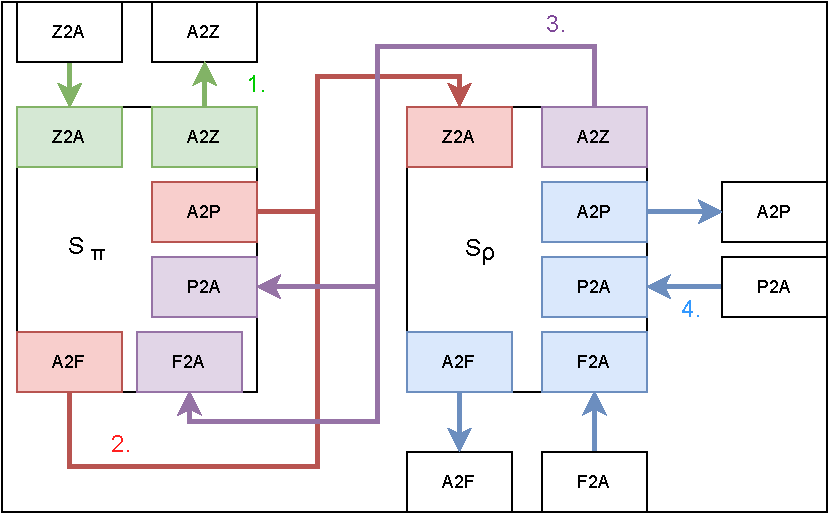
\includegraphics[scale=0.5]{figures/simcomp.pdf}
%\caption{The composed simulators for $\F_1 \xrightarrow{\rho \circ \pi} \F_3$. The real world consists of $(\rho \circ \pi, \F_1)$. Inputs from \Z are for $\F_1$ and dummy parties interacting with $\F_1$, which \SIM{\pi} is equipped to handle. Outputs from \SIM{\pi} are for $\F_2$ and dummy parties of $\F_2$ which \SIM{\rho} is equipped to handle. Finally, outputs from \SIM{\rho} are for $\F_3$ and dummy parties of $\F_3$, which is just the ideal world in Theorem~\ref{thm:composition}.}
%\label{fig:simcomp}
%\end{figure}


\section{Fuzz Testing}
\todo{Still need to mention that we use it to test protocol properties and simulator proofs.}
We rely on fuzz testing as our chosen method of informal protocol analysis for a few critical reasons. 
First, there is a wealth of prior work outlinin the success of fuzz testing techniques, even again program verification, for discovering unintended behavior in code.
Second, existing work in fuzz testing often focuses purely on program binaries that do not concurrently communicate with other processes aside from system calls.
A related work to our own, by Jepsen, takes a novel direction by creating a fuzz testing framework for testing the Tendermint byzantine-fault tolerant consensus protocol. 
Here, several nodes communicate with each other through tcp/ip connections and come to consensus on the ordering of messages sent by all the nodes (refer to Section~\ref{sec:relatedworks} for a more in-depth analysis of the work). 
In this work, we attempt a similar mechanism but constrain ourselves to evaluating protocols expressed in the UC framework.
Furthermore, we replicate the work done by jepsen in our framework as a baseline validation for its capabilities. 

\subsection{QuickCheck in with UC}
The QuickCheck module provides primitives for generating input according to some rules. 
The advatage of modelling protocols within the UC framework is that the interface for the adversary's input to the protocol, and any underlying assumptions or network primitives, is made explicit from the start.
This helps constrain the set of possible inputs give to the adversary and make the framework amenable to fuzzing.

\paragraph{Always Enabled Actions}
Part of defining protocols for fuzz testing in \us requires borrowing an idea from Iron Fleet~\cite{ironfleet}.
In standard UC when ITMs normally halt when something goes wrong.
In agreement protocols, a protocol might ensure distinguishability by simply halting when something incorrect happens such as, for example, receiving a broadcast from a part that isn't the sender or running out of import. 
When writing a protocol in \us it is critical that programs don't throw errors or simply stop accepting messages from others, because such situations lead to test runs that hang indefinitely. 
Instead, all prorams need to ensure that all inputs received from other ITMs result in control being passed to another ITM.
In the case of faults, or halting, this simplifies to passing control back to the environment on any input.  \todo{make this better}


\subsection{Creating Test Cases}

\paragraph{Unstructured Environments}
Creating generative environments that follow some type of protocol ordering requires considerable effort and isn't easily done for protocols that take an arbitrary number of rounds.
For example, a structure protocol like the one described for Braca Broadcast necessarily encodes some number of rounds of inputs that are generated. 
A protocol like ABA or the BenOr protocol break this limitation. 
Therefore, we make a more generalized approach to your fuzz testing were we define try to minimize the protocol assumptions made in our generators and determine
whether we can still capture the same bugs in a reasonable amount of time.
Specifically, we examine whether how ``unstructured`` the generator can be and still produce interesting cases (i.e. those where at least some parties decide on a value) and 
how the weight assigned to different inputs in the generator impact this.
We hypothesized that inputs to our asynchronous wrapper (\texttt{ClockA2F_Deliver} and \texttt{ClockA2F_MakeProgress} commands) must be significantly more frequently generates
than honest party input or corrupt party input in order to ensure that the protocol has a high change of making progress.





\subsection{Discovering Safety Bugs in Protocols}
We examine fuzz testing by implementing some classical and a moden byzantine agreement protocol and injecting faults into them.
Most injected bugs arise from misplaces thresholds for parties to take some action.
For example, a protocol that designed to handle $\frac{n}{2}$  

Most injected bugs arise from misplaced thresholds and incorrect assumptions about corrupt party threstholds. 



\subsection{Analyzing Liveness in Distributed Protocols}
Analysis, even informal, about liveness in protocols is a hard problem.
A large body of existing works, like IronFleet, that uses temporal logic to reason 
about some positive actions happening in a distributed protocol, but this comes at 
the cost of significant user.
In this section we explore to what extend our informal analysis of consensus and agreement
protocols, and our implementation of the import mechanism, can discover and give meaningful
feedback about liveness issues to a protocol analyst.

There are some critical limitations in what an informal analysis can achieve.
With the import mechanism, the most interest kinds are evident when the execution runs out
of import, and this leads to a problem of juggling false negatives and false positives when
asking the question: is this protocol live?
Imagine a probabilistic protocol that makes random decisions
and terminates in some expected number of rounds with byzantine agreement. 
For example, say some execution among the generated test cases outputs an error
that some ITM in the execution is out of import. The error can be explained in one of 
two ways:
\begin{enumerate}
	\item The protocol, as defined, does not get enough import from the environment,  or it doesn't pass around enough import between the parties to achieve the desired functionality. It is a randomized protocol and there may be some sequence of random choices that delays termination by a large enough amount (or for many rounds) that the import provided is insufficient. 
	\item The protocol does have a fault, and there is some sequence of random decisions the parties can make which results in the protocol no terminating in a polynomial amount of time. In reality, regardless of the polynomial import provided, there will always be some sequence of decisions that prevents poly-time termination. 
\end{enumerate}
In fact, it may even be the case that in $n$ generate test cases the faulty traces of an incorrect protocol may never be triggered.  

\paragraph{False Negatives}
False negatives occur when a truly live protocol runs out of import trying to terminate. 
In such cases, the natural next analysis step is increasing the polynomial import given
to the protocol until suc 
\todo{hypothesis is that increasing the polynomial and number of test cases reduces false negatives towards zero at the limit}

\paragraph{False Positives}
individual generated executions that report failures may be false negatives for the reasons above.
A fuzz testing run that returns no failure can be false positive as the failure trace hasn't been discovered. 
\todo{hypothesis is that increasing the polynomial and number of test cases approaches a constant upper bound in the limit as the actual traces with never terminate happen infinitely often}



\section*{Acknowledgment}

\section*{References}

\appendix


\pagebreak

\end{document}
